%!TEX TS-program = xelatex
%!TEX encoding = UTF-8 Unicode

% Figures: full: 174 mm, letters Myriad Variable Concept Regular 16 pt
% half: 85 mm
% Regular type between 10 and 12 pt

\documentclass{Dissertate}

% TODO notes
\definecolor{lightmauve}{RGB}{230,0,230}
\setlength{\marginparwidth}{2.5cm}
\usepackage[textsize=small, linecolor=mauve, bordercolor=black,
            backgroundcolor=lightmauve]{todonotes}
            
\usepackage{wrapfig}

% Scientific notation in text command
\newcommand{\e}[2]{\num{#1}E\num[minimum-integer-digits=2]{#2}}

%hyphenation shorthand
\usepackage[ngerman, english]{babel}
\useshorthands{"}
\addto\extrasenglish{\languageshorthands{ngerman}}

% full page figure
\usepackage{fltpage}

% math non-italic
%\usepackage[LGRgreek]{mathastext}
%\usepackage{mathastext}
\usepackage{upgreek} %text greek letters

% table cells
\usepackage{makecell}

% Environment for methods
\newenvironment{method}
	{
	\vspace{6pt}
	\begin{sffamily}
	\begin{spacing}{\dcompressedspacing}
	\sisetup{detect-all}
	}
	{
	\end{spacing}
	\end{sffamily}
	\vspace{6pt}
	}

% small similar sign
\newcommand{\smallsim}{\smallsym{\mathrel}{\sim}}

\makeatletter
\newcommand{\smallsym}[2]{#1{\mathpalette\make@small@sym{#2}}}
\newcommand{\make@small@sym}[2]{%
  \vcenter{\hbox{$\m@th\downgrade@style#1#2$}}%
}
\newcommand{\downgrade@style}[1]{%
  \ifx#1\displaystyle\scriptstyle\else
    \ifx#1\textstyle\scriptstyle\else
      \scriptscriptstyle
  \fi\fi
}
\makeatother

% same with gtrsim
\newcommand{\smallgtrsim}{\smallgtrsym{\mathrel}{\gtrsim}}

\makeatletter
\newcommand{\smallgtrsym}[2]{#1{\mathpalette\make@small@gtrsym{#2}}}
\newcommand{\make@small@gtrsym}[2]{%
  \vcenter{\hbox{$\m@th\downgrade@style#1#2$}}%
}
\makeatother

% Items more compact
\usepackage{enumitem}

% Box environment
\usepackage{newfloat}
\DeclareFloatingEnvironment[within=none, fileext=frm, placement={!hb}, name=Box]{boxenv}
\captionsetup[boxenv]{font=normalsize, labelfont=bf, textfont=sf} %labelfont %textfont %font ?
\usepackage[framemethod=TikZ]{mdframed}
\definecolor{shadecolor}{RGB}{143,177,196}
\definecolor{dkshadecolor}{RGB}{51,99,125}
\newenvironment{mybox}[1]
    {
    	\begin{boxenv}[!b]
	\begin{small}
    	\begin{mdframed}[
		%roundcorner=5pt, 
		backgroundcolor=shadecolor, 
		linecolor=dkshadecolor,
  		linewidth=4pt,
  		topline=false,
  		rightline=false,
  		leftline=false
		]
    	\caption{#1}
    }
    {
    	\end{mdframed}
	\end{small}
    	\end{boxenv}
    }

% prevent breaking inside LA-N
\usepackage[shortcuts]{extdash}

% siunitx number format
\sisetup{detect-all}

% diagonal fractions
% \usepackage{xfrac}
            
% acronyms
%!TEX root = dissertation.tex
\acsetup{extra-style = paren}

\DeclareAcronym{a7}{
short = CHRNA7,
long = nicotinic acetylcholine receptor subunit $\alpha7$,
class = gene,
sort = chrn
}
\DeclareAcronym{ach}{
short = ACh,
long = acetylcholine,
class = abb
}
\DeclareAcronym{ache}{
short = ACHE,
long = acetylcholinesterase,
class = gene
}
\DeclareAcronym{acly}{
short = ACLY,
long = ATP citrate lyase,
class = gene
}
\DeclareAcronym{ad}{
short = AD,
long = Alzheimer's Disease,
class = abb
}
\DeclareAcronym{ago}{
short = Ago,
long = argonaute,
extra = protein,
class = abb
}
\DeclareAcronym{aif}{
short = AIF1,
long = allograft inflammatory factor 1,
extra = microglia marker protein,
class = gene
}
\DeclareAcronym{api}{
short = API,
long = application programming interface,
class = abb
}
\DeclareAcronym{bche}{
short = BCHE,
long = butyryl cholinesterase,
class = gene
}
\DeclareAcronym{bd}{
short = BD,
long = Bipolar Disorder,
class = abb
}
\DeclareAcronym{bdnf}{
short = BDNF,
long = brain-derived neurotrophic factor,
class = abb
}
\DeclareAcronym{cage}{
short = CAGE,
long = 5' cap analysis of gene expression,
class = abb
}
\DeclareAcronym{chat}{
short = CHAT,
long = choline acetyltransferase,
class = gene
}
\DeclareAcronym{cns}{
short = CNS,
long = central nervous system,
class = abb
}
\DeclareAcronym{cntf}{
short = CNTF,
long = ciliary neurotrophic factor,
class = gene
}
\DeclareAcronym{cntfr}{
short = CNTFR,
long = ciliary neurotrophic factor receptor,
extra = soluble,
class = gene
}
\DeclareAcronym{colq}{
short = COLQ,
long = acetylcholinesterase collagen tail peptide,
extra = ColQ,
class = gene
}
\DeclareAcronym{de}{
short = DE,
long = differentially expressed,
class = abb
}
\DeclareAcronym{dmem}{
short = DMEM,
long = Dulbecco's modified eagle medium,
class = abb
}
\DeclareAcronym{fcs}{
short = FCS,
long = fetal calf serum,
class = abb
}
\DeclareAcronym{fdr}{
short = FDR,
long = false discovery ratio,
class = abb
}
\DeclareAcronym{geo}{
short = GEO,
long = Gene Expression Omnibus,
extra = NCBI,
class = abb
}
\DeclareAcronym{go}{
short = GO,
long = Gene Ontology,
class = abb
}
\DeclareAcronym{gfap}{
short = GFAP,
long = glial fibrillary acidic protein,
extra = central astrocyte marker,
class = gene
}
\DeclareAcronym{gp}{
short = gp130,
long = see IL6ST,
extra = gene,
class = abb
}
\DeclareAcronym{hacu}{
short = SLC5A7,
long = high affinity choline uptake transporter,
extra = also known as HACU,
class = gene
}
\DeclareAcronym{il}{
short = IL\=/6, %extdash package prevents break
long = interleukin 6,
class = gene
}
\DeclareAcronym{ilr}{
short = IL6R,
long = interleukin 6 receptor,
extra = soluble,
class = gene
}
\DeclareAcronym{ilst}{
short = IL6ST,
long = interleukin 6 signal transducer,
extra = membrane bound; also known as gp130,
class = gene
}
\DeclareAcronym{jak}{
short = JAK,
long = janus kinase,
class = gene
}
\DeclareAcronym{la2}{
short = LA\=/N\=/2, %extdash package prevents break
long = human neuroblastoma cell line,
extra = female,
class = abb
}
\DeclareAcronym{la5}{
short = LA\=/N\=/5, %extdash package prevents break
long = human neuroblastoma cell line,
extra = male,
class = abb
}
\DeclareAcronym{lif}{
short = LIF,
long = leukaemia inhibiting factor,
class = gene
}
\DeclareAcronym{lifr}{
short = LIFR,
long = leukaemia inhibiting factor receptor,
extra = soluble,
class = gene
}
\DeclareAcronym{loo}{
short = LOO,
long = Leave-One-Out,
extra = approach,
class = abb
}
\DeclareAcronym{mir}{
short = miRNA,
long = microRNA,
class = abb
}
\DeclareAcronym{ngfr}{
short = NGFR,
long = nerve growth factor receptor,
extra = also known as p75,
class = gene
}
\DeclareAcronym{nt}{
short = nt,
short-plural-form = nt,
long = nucleotide,
class = abb
}
\DeclareAcronym{ntrk1}{
short = NTRK1,
long = neurotrophic receptor tyrosine kinase 1,
class = gene
}
\DeclareAcronym{ntrk2}{
short = NTRK2,
long = neurotrophic receptor tyrosine kinase 2,
class = gene
}
\DeclareAcronym{ncbi}{
short = NCBI,
long = National Center for Biotechnology Information,
class = abb
}
\DeclareAcronym{ngf}{
short = NGF,
long = nerve growth factor,
class = gene
}
\DeclareAcronym{oli}{
short = OLIG1,
long = oligodendrocyte transcription factor 1,
class = gene
}
\DeclareAcronym{or}{
short = OR,
long = odds ratio,
class = abb
}
\DeclareAcronym{pbs}{
short = PBS,
long = phosphate buffered saline,
class = abb
}
\DeclareAcronym{pcr}{
short = RT\-/qPCR, %extdash package allows break
long = real-time quantitative polymerase chain reaction,
class = abb
}
\DeclareAcronym{pd}{
short = PD,
long = Parkinson's Disease,
class = abb
}
\DeclareAcronym{prima}{
short = PRIMA1,
long = proline-rich membrane anchor 1,
class = abb
}
\DeclareAcronym{rbf}{
short = RBFOX3,
long = RNA-binding Fox-1 homolog 3,
extra = neuronal marker gene; also known as NeuN,
class = gene
}
\DeclareAcronym{rin}{
short = RIN,
long = RNA integrity number,
extra = RNA quality measure,
class = abb
}
\DeclareAcronym{risc}{
short = RISC,
long = RNA-induced silencing complex,
class = abb
}
\DeclareAcronym{rpmi}{
short = RPMI1640,
long = Roswell Park Memorial Institute medium,
class = abb
}
\DeclareAcronym{scz}{
short = SCZ,
long = Schizophrenia,
class = abb
}
\DeclareAcronym{seq}{
short = RNA-seq,
long = RNA sequencing,
class = abb
}
\DeclareAcronym{slc}{
short = SLC18A3,
long = vesicular acetylcholine transporter,
extra = official gene symbol,
class = gene
}
\DeclareAcronym{smrna}{
short = smRNA,
long = small non-coding RNA,
class = abb
}
\DeclareAcronym{sql}{
short = SQL,
long = structured query language,
class = abb
}
\DeclareAcronym{sst}{
short = SST,
long = somatostatin,
class = gene
}
\DeclareAcronym{stat}{
short = STAT,
long = signal transducer and activator of transcription,
class = gene
}
\DeclareAcronym{tf}{
short = TF,
long = transcription factor,
class = abb
}
\DeclareAcronym{trf}{
short = tRF,
long = transfer RNA fragment,
class = abb
}
\DeclareAcronym{tirna}{
short = tiRNA,
long = transfer RNA half,
long-plural-form = transfer RNA halves,
class = abb
}
\DeclareAcronym{tpm}{
short = TPM,
long = transcripts per million,
class = abb
}
\DeclareAcronym{trna}{
short = tRNA,
long = transfer RNA,
class = abb
}
\DeclareAcronym{tyk}{
short = TYK,
long = tyrosine kinase,
class = gene
}
\DeclareAcronym{utr}{
short = UTR,
long = untranslated region,
class = abb
}
\DeclareAcronym{vacht}{
short = vAChT,
long = vesicular acetylcholine transporter,
extra = from SLC18A3 gene,
class = abb
}
\DeclareAcronym{vip}{
short = VIP,
long = vasoactive intestinal peptide,
class = gene
}



\begin{document}

% the front matter
%!TEX root = ../dissertation.tex
% Some details about the dissertation.
\title{Small RNA dynamics in cholinergic systems}
\author{Sebastian Lobentanzer}

%If you have one advisor
\advisor{Jochen Klein}

%If you are coadvised
\coadvisorOne{Hermona Soreq}

% Everyone has an External committee member
\committeeExternal{Person Outside}

% ... about the degree.
\degreeyear{2019}

% \maketitle
% \copyrightpage
\frontmatter
\renewcommand{\chapterheadstartvskip}{\vspace*{-0.5\baselineskip}} %this shifts chapter headlines vertically
\setstretch{\dnormalspacing}
% \abstractpage
% \tableofcontents
% %\authorlist
% \listoffigures
% \dedicationpage
% \acknowledgments

% \doublespacing


% include each chapter...
% \setcounter{chapter}{-1}  % start chapter numbering at 0
%!TEX root = ../dissertation.tex
\begin{savequote}[75mm]
I know words. I have the best words.
\qauthor{Donald Trump}
\end{savequote}

\chapter{Introduction}
\label{introduction}
\section{Cholinergic Systems}
\newthought{Nary a process in the mammalian body can commence without participation of cholinergic systems.} \Ac{ach} was chemically and pharmacologically described by Henry Dale more than 100 years ago\cite{Dale1914}. A short time later, Otto Loewi published the first proof of signal transmission by small molecules: he transferred physiological solutions from electrically stimulated frog hearts to naive hearts and observed their reactions; the solution that provoked a parasympathetic response he proposed to contain a »vagus substance«\cite{Loewi1921}. Finally, in 1929, Henry Dale completed the picture by isolating acetylcholine from mammalian tissue and identifying it as the molecule responsible for the parasympathetic response\cite{Dale1929}. Dale and Loewi's joint effort in »Discoveries in Chemical Transmission of Nerve Impulses« was rewarded with the Nobel Prize in Physiology or Medicine in 1936.

Although we have learned much about cholinergic systems in these past 100 years, our understanding of the mammalian nervous system still is fairly limited. Even when disregarding peripheral nervous systems, the complexity of cholinergic transmission is immense, and a myriad of functions have been attributed to cholinergic circuits in the \ac{cns}. Central nervous projections of cholinergic fibres were extensively mapped by M. Marsel Mesulam and others in the 1980s\cite{Mesulam1984}, with a majority of long projection neurons originating in one of the eight cholinergic nuclei, Ch1-Ch8. While many of these anatomical structures have been filled with meaning by associations with both rudimentary as well as higher brain functions, there are still as many cholinergic pathways whose function is entirely unclear (Figure \ref{fig:projections}, from my first manuscript\cite{Lobentanzer2019a}).

This holds particularly true for the only recently discovered cortical cholinergic interneurons, which, in comparison to their projecting counterparts, are very small and numerically vastly inferior to other neuron types in the cortex. Thus, their detection and analysis with current methods is challenging. 

\begin{figure}
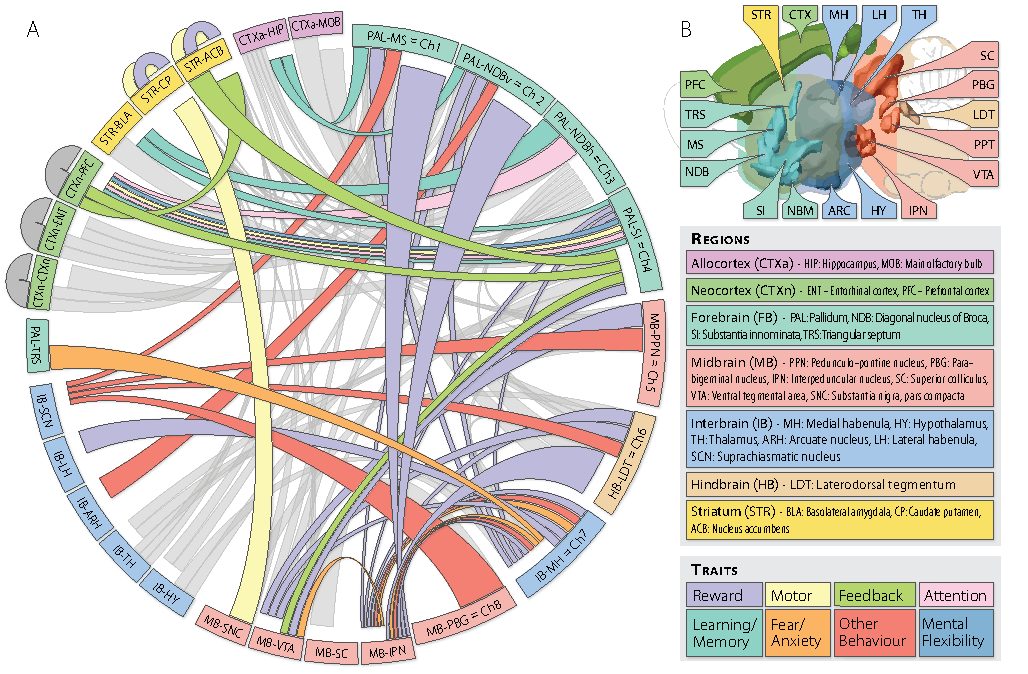
\includegraphics[width=\textwidth]{figures/projections}
\caption[Short figure name.]{This is a figure that floats inline and here is its caption.
\label{fig:projections}}
\end{figure}

\subsection{Cholinergic Aspects of Disease}
\newthought{Since cholinergic systems are integral for a myriad physiological functions}, they are naturally involved in aetiologies and phenotypes of a number of central and peripheral diseases. Of interest to this dissertation are the cholinergic aspects of degenerative and non-degenerative central nervous diseases (such as Alzheimer's Disease, Bipolar Disorder, Schizophrenia), ischemic conditions in stroke, and peripheral modulation of immune responses, particularly in the context of the aforementioned diseases.

\subsubsection{Alzheimer's Disease}
Cholinergic progression

Monotherapeutic approaches

\subsubsection{Schizophrenia and Bipolar Disorder}
Dirty therapeutics, multitarget

\subsubsection{Stroke}

\subsubsection{Immunity}

\subsection{Neurokines}
In comparison to the widely studied cholinergic projection neurons originating in the basal forebrain (Ch1-Ch4) that are known to depend on a retrograde survival signal by means of \ac{ngf}, trophic influences on other cholinergic populations such as the cortical interneurons are unclear.  \ac{ngf} was described by Rita Levi-Montalcini in the 1950s as the first known instance of trophic peptides required for the survival of sympathetic ganglia\cite{Levi-Montalcini1960}, and the dependence of basal forebrain cholinergic neurons on retrograde \ac{ngf} signalling was discovered in the 1980s\cite{Hefti1986}.

A second group of trophic peptides with cholinergic implications are the so-called »neurokines«; the name results from the fact that this particular subgroup of cytokines has been associated with neuronal function in the central and peripheral nervous systems. Most prominently they include the \ac{cntf}, \ac{lif}, and \ac{il}, all of which coincidentally have been known under the acronym CDF. In the end of the 1980s, two groups of scientists (McManaman\cite{McManaman1988} and Rao\cite{Rao1992}) independently identified proteins in extracts of muscle fibre that induced a differentiation of neurons towards a cholinergic type, and thus termed these proteins »choline acetyltransferase development factor« or »cholinergic differentiation factor« (both abbreviated CDF). Only later, through sequencing of the peptides, it became known that they had in fact discovered two distinct neurokines, \ac{lif} (Rao) and \ac{cntf} (McManaman, personal communication). \ac{il}, on the other hand, is abbreviated CDF for an entirely different reason: in this case it is short for »CTL (cytolytic T lymphocyte) differentiation factor«.

\ac{cntf}, \ac{lif}, and \ac{il} convey their impact on neuronal activity through a partly redundant neurokine receptor pathway. There are two basic types of neurokine receptors: soluble and transmembrane. The primary receptors for \ac{cntf} (\acs{cntfr}) and \ac{il} (\acs{ilr}) are soluble proteins that are secreted into the extracellular space and, upon binding of a neurokine, bind to transmembrane receptor dimers on the cell surface. These transmembrane receptors are the LIF receptor (\acs{lifr}) and the »interleukin 6 signal transducer« (\acs{ilst}, also known as \acs{gp}). Every neurokine has its preferred constellation of soluble and transmembrane receptors: \ac{cntf} binds to the soluble \ac{cntf} receptor and a dimer consisting of one \ac{gp} and one \ac{lifr} protein; \ac{il} binds to the soluble IL6R and a dimer of two units of \ac{gp}; \ac{lif} does not usually bind a soluble receptor but rather binds immediately to a dimer comprising one of each \ac{gp} and \ac{lifr}; however, there is significant redundancy and crosstalk between those systems\cite{Rawlings2004,Nathanson2012}.

All receptor constellations result in a main effect of activation of the \acs{jak}/\acs{stat} cascade (Fig. \ref{fig:neurokine}). More specifically, neurokines can activate \acfp{jak} 1 and 2 or the homologous \ac{tyk} 2, and, successively, \ac{stat} (»signal transducer and activator of transcription«) isoforms 1, 3, 5A, and 5B, which then convey a multitude of cellular effects (e.g. in immunity or differentiation) through transcriptional activation. The \ac{stat} cascade is inherently self-limiting in that it usually leads to expression of transcription factors that serve as repressors of the \ac{stat} genes (XXX)\cite{}. 

Neurokines, particularly \ac{il}(?), might serve as a link between the immunological and cholinergic aspects of physiological or disease processes.\todo{find a place}

\begin{figure}
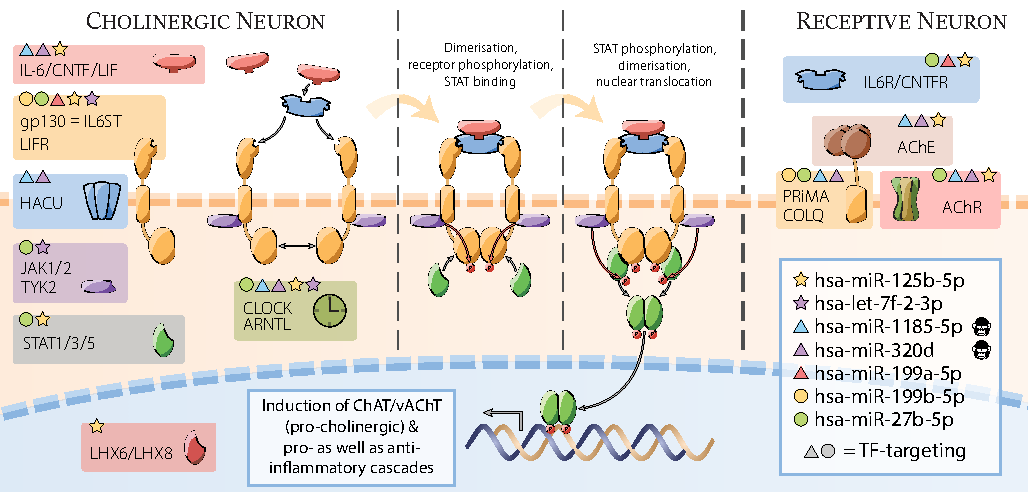
\includegraphics[width=\textwidth]{figures/neurokine}
\caption[Short figure name.]{This is a figure that floats inline and here is its caption.
\label{fig:neurokine}}
\end{figure}

%Neuronal activity is profoundly modified by cytokines

%Li Gan - NFkB activation by tau
% - Ikkbeta knockout corrects STAT1 DE

%Oleg Butovsky - TGFbeta as master glia regulator

\section{Transcriptional Connectomics}
The term »connectomics« is not strictly limited to one scientific discipline; it is frequently used when the studied matter is defined by complex relationships between interaction partners; the most frequent use outside of transcriptional matters is neuronal connectomics, i.e., the relationships and projections between brain regions. In this dissertation, connectomics generally refers to epi-transcriptional interaction, the processes surrounding protein-coding gene expression. For the sake of simplicity, all descriptions of genomics and transcriptomics matters, genes, \acp{mir}, and tRFs in this dissertation are to be seen in the context of \textit{Homo sapiens}, unless explicitly stated otherwise.

\newthought{No matter their location, cholinergic neurons are defined by their ability to synthesise \ac{ach} and release it to neighbouring cells to a certain effect.} To fulfil this task, two particular proteins are essential: the \ac{chat} to synthesise \ac{ach} from choline and acetyl-Coenzyme A, and the vesicular acetycholine transporter (\acs{vacht}, official gene symbol \acs{slc}), which concentrates \ac{ach} in vesicles for later release. A notable genetic feature connects these two proteins beyond their functional association: the small \textit{\ac{slc}} gene (2420 nucleobases) sits inside the first intron of the \textit{\ac{chat}} gene and thus is already included in its primary transcript, and is subject to the \textit{\ac{chat}} promoter. However, oftentimes the (mature) transcript levels of \textit{\ac{chat}} and \textit{\ac{slc}} mRNA seem to be independently regulated; from the perspective of the organism, the possibility of differential regulation between these two genes makes sense. Since \textit{\ac{slc}} does not possess its own promoter, this differential regulation has to be conveyed epigenetically. 

This dissertation deals in large parts with approaches aiming to decipher these interactions; and while its primary topic revolves around cholinergic systems, the methods described in the following are designed to be applicable to the entirety of the genome/epigenome. Four particular types of cellular actors are subject of these methods and therefore will be briefly introduced: genes in the classical sense as the conveyors of cellular function by encoding for proteins; \acp{tf}, a subclass of protein coding genes that are able to regulate the expression of other genes; \acp{mir}, a class of small non-coding RNA that has been known for approximately two decades and is reasonably well described functionally and mechanistically; and \acp{trf}, a second class of small non-coding RNA that has only recently been rediscovered and is significantly less well described regarding its functionality.

\subsection{Transcription Factors} \label{sec:intro:tf}
\Acp{tf} were among the first intracellular regulatory mechanisms to be discovered (the earliest article referencing the term »transcription factor« in its title on PubMed was published in 1972). \acp{tf} commonly translocate from the cytosol into the nucleus upon activation (often by phosphorylation), where they bind specific DNA sequences that usually range in size from 6 to 12 nucleobases. The regions containing these binding sites (about 100 - 1000 bases in size) determine the effect upon binding, which can be one of two main modes: either a promoter, leading to an increased activity of transcription in the downstream vicinity of the binding site, or a repressor, having the opposite effect. 

There exists a vast body of knowledge on \ac{tf} interactions with genes, mostly due to the long period of time since their discovery and the multitude of scientific publications, most often studying single \acp{tf} and their interactions with few genes, but cumulatively curated by several organisations. One of the currently largest curations of \ac{tf} data, TRANSFAC, saw its original release in 1988. While these curation efforts can be extensive, they may present with serious bias towards particular \acp{tf} that might hold more scientific interest and thus are published far more frequently than others. Recently, comprehensive efforts have extended the available data significantly. Driven by the advent of \ac{seq}, computational approaches have become able to not only comprehensively predict \ac{tf}-gene interactions, but to do so in a highly tissue-specific manner (see \ref{sec:database:tf}). The human body is estimated to express up to 2600 distinct DNA-binding proteins, most of them presumed \acp{tf}\cite{Babu2004}, although other studies give lower estimates. 

\subsection{microRNAs} \label{sec:intro:mirna}
\newthought{The first endogenous »small RNA with antisense complementarity«} was described in 1993\cite{Lee1993}, but \acp{mir} were only recognised as a distinct regulatory class of molecules in the early 2000s. They are typically between 18 and 22 nucleobase-long, single stranded RNA fragments, and their function is now largely undisputed: \acp{mir} serve as targeting molecules for a protein complex whose primary purpose is to repress translation of mRNA, and, in some cases, lead to mRNA degradation. The complex, therefore, is called \ac{risc}; central to its function is the family of \ac{ago} proteins, which can bind the mature \ac{mir} and orient it for interaction with its targets. Guidance of \ac{risc} to the target mRNA is generally mediated via sequence complementarity between \ac{mir} and the targeted mRNA. Specifically, a »seed« region, usually bases 2-8 on the \ac{mir}, is mainly responsible for the interaction; in case of perfect complementarity of this seed to the mRNA sequence, the interaction is considered »canonical«.

In early \ac{mir} research, the 3' \ac{utr} of the mRNA was believed to contain most \ac{mir} binding sites due to its greater accessibility (i.e., the lack of active ribosomes); however, cumulative recent reports suggest that binding inside the coding region of the mRNA is a regular occurrence(cite). The rules governing \ac{mir} binding to target sequences show considerable flexibility; a recent study shows about 30\% of analysed relationships to be of »non-canonical« nature(cite). In those cases, seed pairing with the mRNA is often imperfect. To ameliorate this loss of stability, compensation occurs typically by a secondary complementary structure after a small gap of non-complementary bases, leading to a »bridge«-type constellation. \todo{FIGURE?} This flexibility has implications in applications involving targeting algorithms; those that consider only the seed region are more prone to false negatives than models that consider, for instance, the free energy of the whole molecule (see \ref{sec:database:mirna}).

\subsubsection{Biogenesis}
\acp{mir}, similar to coding genes, are transcribed from loci on the genome, many inside introns or even exons of coding genes\cite{Rodriguez2004}. The primary transcript (primary \ac{mir} or pri-\ac{mir}) typically contains a hairpin-like structure that usually results in a double-stranded molecule because of internal complementarity, and can contain up to six mature \acp{mir}. This hairpin structure is recognised by the DGCR8 protein (DiGeorge Syndrome Critical Region 8, in invertebrates called »Pasha«); the complex then associates with the RNA-cleaving protein »Drosha«, which removes bases on the opposite side of the hairpin, creating a \ac{mir} precursor (or pre-\ac{mir}), which is subsequently exported from the nucleus by the shuttle protein Exportin-5. In a final step in the cytosol, the ribonuclease »Dicer« removes the loop joining the 3' and 5' arms of the pre-\ac{mir}, resulting in a duplex of mature \ac{mir}, about 20 nucleotides long. Initially, it was thought to contain only one active \ac{mir}, resulting in a designation of »\ac{mir}*« for the complementary strand (commonly, the strand with lower expression). However, this notion has been disproven, and to reflect the possibility of both strands performing \ac{mir} functions, nomenclature has changed to specify the arm of the pre-\ac{mir} from which the mature form originates (suffix »-3p« for the 3' arm, and »-5p« for the 5' arm).

\ac{mir} genes, in the same way as protein coding genes, can be subject to promoters and repressors, adding another layer of expression control by \acp{tf}. However, these \ac{tf}-\ac{mir} relationships are far less well described than common coding gene interactions, because \acp{mir} due to their shortness are not amenable to many standard gene expression assay forms. Estimation of the number of distinct targets of any one \ac{mir} varies widely; however, it is generally accepted to not be less than several dozen targets per \ac{mir}, and up to thousands of genes per \ac{mir} (although that estimate might be overenthusiastic).

\subsubsection{Organisation and Curation}
\acp{mir} are organised and curated by means of a periodically updated web-based platform, miRBase\cite{Kozomara2019}. For \textit{Homo sapiens}, miRBase v21 contains 2588 mature \acp{mir} from XXX precursors. Evolutionarily, the \ac{mir} repertoire has grown from rodents to primates, resulting in a number of primate-specific \acp{mir} that may convey additional function. \ac{mir} nomenclature is organised\cite{Ambros2003} in a way that assigns evolutionarily conserved \acp{mir} the same designation (number) in all species in which they are expressed. In their full names, a prefix stating the organism of origin is added; for example, hsa-miR-125b-5p (for \textit{Homo sapiens}) and mmu-miR-125b-5p (for \textit{Mus musculus}) share the same sequence and most of their functionalities.

\acp{mir} are subcategorised in families (designated »mir« with lowercase »r«) by their genomic origin and phylogenetic homology aspects. As the annotation itself, family affiliations are in flux and change with each miRBase version. miRBase v21 lists 151 distinct \ac{mir} families with XX individual members in total. The remaining XX \acp{mir} do not belong to a larger family.

\subsubsection{Disease Association}
\acp{mir} have been associated with a number of \ac{cns} diseases, including \ac{ad}, \ac{pd}, \ac{bd}, and \ac{scz}. However, the largest contribution since their discovery by far has been made by cancer research; of the approximately \num{90000} publications found on PubMed with the term \ac{mir}, about \num{42000} involve cancer (search term »\ac{mir} AND cancer«). In comparison, »\ac{mir} AND Alzheimer's Disease« results in about 600 hits, while a search for »\ac{mir} AND Schizophrenia« yields just 363 publications (as of October 2019).

In \ac{ad}, several groups of \acp{mir} have been found to show characteristic perturbations before the onset of symptoms, which makes them interesting biomarker candidates\cite{Salta2017a}. Some \acp{mir} have been extensively studied in a variety of contexts, most prominently hsa-miR-132-3p. Among its targets are several key neuronal regulators (e.g. FOXP2, FOXO3, P300, MeCP2), and it is in turn controlled by many pivotal neuronal elements (e.g. REST, ERK1/2, CREB)\todo{add to abbreviations?}; this presents an explanation for the many physiological and pathological situations that miR-132-3p has been found to play a role in. Its functions include the control of neuronal survival/apoptosis, migration and neurite extension, neuronal differentiation, and synaptic plasticity. 

\acp{mir} are able to fulfil their regulatory purpose in a context- and cell-type-dependent manner\cite{Lu2015}, such that the perturbation of one single \ac{mir} might provide different functional outcomes in different tissues (e.g., glial cells and neurons), or different stages of disease.

\todo{Prediction?}

\subsection{Transfer RNA Fragments}
\newthought{\Ac{trna} breakdown products have been known for decades}, with first descriptions in the 1970s; back then, they were associated with a higher turnover of \ac{trna} in cancer cells\cite{Borek1977}, and proposed as urine-based biomarkers for certain malignancies\cite{Speer1979}. However, their genesis was attributed to random processes, and due to lacking molecular biology characterisation techniques, interest in those fragments quickly faded. It was not until recently that studies have shown \ac{trna} to be a major source of stable expression of small noncoding RNA\cite{Cole2009,Lee2009} in most mammalian tissues. Indeed, replicating the reports from the 1970s, \ac{trna} breakdown products are the dominant form of small RNA in secreted fluids, such as urine and bile, and make up large parts of other bodily fluids as well\cite{Godoy2018}. They exist in two major forms: \acp{tirna}, and the smaller \acfp{trf}. \textit{from stroke paper} \acp{tirna} derive from either end of the \ac{trna}, and are created by angiogenin cleavage at the anticodon loop\cite{Yamasaki2009,Ivanov2011}. Smaller fragments are derived from the 3’ and 5’ ends of the \ac{trna} (3'-\ac{trf}/5'-\ac{trf}) or internal \ac{trna} parts (i-\ac{trf}), respectively, and may incorporate into \ac{ago} protein complexes and act like \acp{mir} to suppress their targets\cite{Burroughs2011,Kumar2014}.

However, there is considerable controversy about the generalisation of \ac{trf} functions, as distinct publications discover very different and sometimes opposing mechanisms of action for their respective fragments. An obvious assumption is the \ac{mir}-like functionality, at least for those \acp{trf} that are in the length range of \acp{mir}. There have been several instances of \acp{trf} proven to act as \ac{mir}-like suppressors of translation in a \ac{risc}-associated manner\cite{Kumar2014}, and of Dicer playing a large part in their biogenesis\cite{Cole2009}. There are even instances of small RNA molecules previously mislabeled \acp{mir} that have been discovered to actually be \ac{trna}-derived, such as miR-1280\cite{Huang2017}.

On the other hand, multiple groups have identified \acp{trf} to function not in an antisense-complementary manner, but by homology aspects. A valine-derived \ac{trf} was found to regulate translation by competing with mRNA directly at the binding site at the initiation complex and thereby displacing the original mRNA, leading to its translational repression\cite{Gebetsberger2017}. Others have found multiple classes of \acp{trf} derived from glutamine, aspartate, glycine, and tyrosine \acp{trna}, that displace multiple oncogenic transcripts from an RNA-binding protein (YBX1), conveying tumor-suppressive activity\cite{Goodarzi2015}. Most counterintuitive is the recent finding of a \ac{trf} proven to bind to several ribosomal protein mRNAs and enhancing their translation, and, when specifically inhibited, leading to apoptosis in rapidly dividing cells\cite{Kim2017}.

There is no consistent nomenclature yet to describe and organise \acp{trf}, which are by nature more heterogeneous than \acp{mir}; considering their biogenesis, one \ac{trna} molecule can be the origin of several hundred distinct \ac{trf} molecules. Multiple approaches are common in current literature, most prominently \acp{trf} are tied to the parent \ac{trna} and the amino acid coded for by this \ac{trna}. For example, the 22-nucleotide-long LeuCAG3′ \ac{trf} (meaning: a fragment of 22 bases starting at the 3' end of the leucine-carrying \ac{trna} with anticodon »CAG«) was shown to play an important role in regulating ribosome biogenesis\cite{Kim2017}. Since there is no repository of the likes of miRBase yet, this approach can be cumbersome for replication purposes, and explicit statement of the exact sequence of each fragment is a must in publication. In fact, since the aforementioned paper does not mention the sequence explicitly, there exist 6 distinct possibilities of fragments fitting this description. While manageable on this small scale, this system prohibits efficient analysis of larger sets of \acp{trf} that cannot be individually controlled. For this reason, the approach of Loher and colleagues\cite{Loher2017} might be preferable: they propose the generation of a "license plate" based on the sequence of the fragment directly, composed of the prefix »\ac{trf}«, the length of the fragment, and a custom oligonucleotide string encoding (e.g., »B3« stands for »AAAGT«). This way, \ac{trf} names are unique and unmistakably linked to the sequence, nomenclature is species-independent, and \ac{trna} origin can be quickly determined by sequence lookup.

\todo{Disease?}

? Levels of \acp{trf} may be modulated even more rapidly than levels of \acp{mir}, since \ac{trna} molecules are very abundant in the cell and generation of mature \acp{trf} requires only enzymatic degradation of \ac{trna} but no de-novo transcription of the molecule in the nucleus (citation).

\section[Nested Multimodal Transcriptional Interactions - The Need for Connectomics]{\nopagebreak{Nested Multimodal Transcriptional Interactions\\ \qquad \qquad - The Need for Connectomics}}
The ultimate aim of transcriptional connectomics is the combination of all interacting cellular components in a model that satisfactorily explains our real-life observations, and is able to predict the functional outcome of a modification of one of these players. Even in the simplified case of only studying the interactions between coding genes, \acp{tf}, \acp{mir}, and \acp{trf}, the complexity of the required model exceeds our current capabilities by far. The more we know about the functioning of these intertwined systems, the more we understand how much there is still to learn. 

For example, only recently has it become clear how complex transcriptional regulation by means of \acp{tf} really is, and, incidentally, the two systems studied foremost in this dissertation (nerve and immune cells) are the two most transcriptionally complex systems in any mammal. Through study of comprehensive genomic information of 394 tissue types in approximately 1000 human primary cell, tissue, and culture samples (from the FANTOM5 consortium) it was estimated that the mean number of active \acp{tf} towards any given gene is highest in immune (12 \acp{tf} per gene) and nervous cells (10 \acp{tf} per gene), and that any one \ac{tf} in nervous and immune cells controls expression of a mean of 175 and 160 genes, respectively\cite{Marbach2016} (see also Section \ref{sec:database:tf}). 

Similarly, it has been found that \acp{mir}, particularly in the nervous system, possess a much higher tissue specificity than coding genes, resulting in an expression landscape that varies widely between individual neuron types that are in close proximity in the brain. With the exception of single cell \ac{seq}, no modern analysis method is capable of a resolution appropriate for accurate characterisation of these expression patterns, resulting in extinction of the signal of \acp{mir} that are not expressed consistently across cell types (similar to »housekeeping« genes) because of statistical interference. Very recent studies show that \ac{mir}-gene co-expression networks are tightly linked to cell types in the nervous system, and that groups of miRs as functional modules associate with particular phenotypes in developmental and mature states\cite{Nowakowski2018}. This functional association with cell phenotype was found in quality comparable to the expression patterns of \acp{tf}, yet in quantity conveys smaller impact and thus is thought to be a fine-tuning mechanism, subtle and precise in purpose. 

Another aspect of the tissue specificity of \ac{cns}-associated \acp{mir} is the high likelihood of under-representation or even non-discovery of those very specifically expressed \acp{mir}. Adding to the problem is the experimental bias towards rodent models when it comes to thorough studies of the \ac{cns}, where human or other primate samples are a rarity compared to rats or mice. Assessments of the numbers of yet unknown novel primate- and tissue specific \acp{mir} estimate their magnitude in the thousands\cite{Londin2015}, resulting in an effective doubling of currently known \acp{mir}.

These high numbers of potentially interacting players present computational challenges: If estimating the number of expressed genes in a human cell at \num{20000} (and the number of \acp{tf} at a low 1000), this makes for an estimated minimum of \num{200000} »real« interactions in the possible $ C = \frac{1000!}{10!(1000-10)!} \cdot \num{20000} $, which practically equals infinity; this is without accounting for different tissue types or cell states (e.g., differentiation or disease). Similarly, the amount of mature \acp{mir} (2588 in miRBase v21) and their ability to target even more distinct transcripts than \acp{tf} with one single molecule present immense computational requirements for even listing all possible or actual relationships. An interaction table describing targeting of genes by \acp{mir} in one type of tissue has $ 2588 \cdot \num{20000} \approx \num{50000000} $ individual fields.

Combining the different modes of transcriptional interaction presents additional challenges. A simple model system to visualise (in only one type of cell) the interaction of \acp{tf} targeting genes, and of \acp{mir} targeting genes as well as \acp{tf}, contains about \num{20000} genes (a subset of which of the size of about 2000 are \acp{tf}), 2588 mature \acp{mir}, and a total of $ 2588 \cdot \num{20000} + 2000 \cdot \num{20000} \approx \num{90000000} $ potential interactions. In standard application scenarios, such as the generation of an interaction network around a group of genes (e.g., the cholinergic genes), the processing requirements grow linearly with each added interaction partner, and exponentially with every regulatory layer that is added. \todo{example of standard interaction gene x miR x TF}

Practically, this information has to be provided, gathered, and integrated, which further multiplies the amount of storage and processing power required. miRWalk 2.0, a collection of \ac{mir} interaction data, has collected 12 of the most popular \ac{mir}-targeting prediction datasets, each of which has their strengths and weaknesses (see \ref{sec:database:mirna}). Experimentally validated interactions (e.g. as collected in DIANA TarBase or miRTarBase) are gold standard, but far from comprehensive and strictly speaking only relevant for the cellular context in which the experiment was originally performed; there are also different evidence qualities to be accounted for, depending on the type of experiment performed. Ideally, all of these data are still accessible when performing the analysis, so a database created for this purpose should be able to incorporate all this information without any data loss while still remaining feasible in terms of computation time as well as space and working memory requirements. 

This dissertation will first describe the creation of such a database and what has been learned during its various stages, and then go on to apply the database to different biological problems from real world experiments, such as the cholinergic differentiation of human male and female cultured neuronal cells, and the blood of stroke victims.
%insert blank page
\newpage\null\pagestyle{plain}\newpage

% header with section title
\pagestyle{fancy}
\fancyhf{}
\renewcommand{\sectionmark}[1]{\markright{#1}} %no number
\fancyhead[le,ro]{\nouppercase{\rightmark}}
\fancyfoot[le,ro]{\thepage}
\renewcommand{\headrulewidth}{.4pt}
\renewcommand{\footrulewidth}{.4pt}

%!TEX root = ../dissertation.tex
\begin{savequote}[75mm]
»Wir sehen in der Natur nie etwas als Einzelheit, sondern wir sehen alles in Verbindung mit etwas anderem, das vor ihm, neben ihm, hinter ihm, unter ihm und über ihm sich befindet.«
\qauthor{Johann Wolfgang von Goethe}
\end{savequote}

\chapter[miRNeo: Creation of a Comprehensive Connectomics Database]{miRNeo: Creation of a\\Comprehensive Connectomics Database} \label{sec:database}
Natural philosophy, as represented by the thought of Johann Wolfgang von Goethe, wants to holistically describe nature and explain and interpret its particular mechanisms. Although natural philosophy is the predecessor of modern, empirical science, its concepts and approaches are still valuable in today's data driven world. As the data we collect grows to dimensions that can only be interpreted with the aid of computers, functional reductionism becomes a valuable paradigm: By studying the facets of nature, we strive to understand it as a whole. Similarly, we regularly encounter Goethe's paraphrase of »all things are connected« in neuro-immunology, and in transcriptional connectomics.

\newthought{Bioinformatic support in connectomics} is indispensable, which can be seen by the sheer multitude of possible interactions between the participating factors. However, when I began working on this project (October 2015), there was no integrative database available for this purpose. Earlier that year, miRWalk 2.0 had been published, for the first time providing a relatively comprehensive source of predicted as well as experimentally validated \ac{mir} targeting data\cite{Dweep2015} (see \ref{sec:intro:mirna}). One year later, Marbach's »regulatory circuits« were published,\cite{Marbach2016} enabling analysis of comprehensive \ac{tf}$\to$gene relationships in 394 human tissues (see Section \ref{sec:intro:tf}). These collections (as well as the data they were derived from) are the basis of the database further called \textit{miRNeo}, the development of which will be described in the following chapter.

Since a large part of the scientific progress of this dissertation deals with practical problems of multimodal connectomics, I will begin by describing the infrastructure that makes effective computation of these problems possible. After this technical description of database structure and creation, I will explain the types and organisation of its content. The remainder of the chapter will then deal with the application of this infrastructure to real-world problems in transcriptional connectomics, and the statistical approaches suited to this special case.

%%%%%%%%%%%%%%%%%%%%%%%%%%%%%%%%%%%%%%%%%%%%%%%%
%%%%%%%%%%%%%%%%%%%%% SECTION %%%%%%%%%%%%%%%%%%%%%
%%%%%%%%%%%%%%%%%%%%%%%%%%%%%%%%%%%%%%%%%%%%%%%%

\section{miRNeo - Implementation}
For any biological question to be asked in a bioinformatics setting, the effectiveness of the computational query determines the practicality of the approach. Because resources (i.e., processing power, storage, and working memory) are limited, the database that is queried should be organised in a way that facilitates retrieval of the desired information without excess processing of useless information, for instance, reporting the absence of a connection. In the simplified case of only \acp{mir} interacting with genes in one direction (\ac{mir}$\to$gene), this means retrieval of only those interactions relevant for the queried genes or \acp{mir}. 

Traditional table-based approaches (also known as relational databases) such as \acs{sql}  (»Structured Query Language«) cannot provide such an implementation, since individual entries for genes and \acp{mir} (rows and columns) have to be accessed in their entirety, whether there is a connection between gene and \ac{mir} (1) or not (0). Additionally, adding layers to these interactions (e.g., distinct prediction algorithms, tissues, or the interaction between \acp{tf} and genes) require the addition of entire tables the same size as the database, which is detrimental to effective use of space; and more complex queries also necessitate the transfer of information between those distinct tables (in \ac{sql} typically via a \textcolor{dkblue}{JOIN} command), which claims additional working memory and processing time. Overall, the so-called »many-to-many« organisation of data does not lend itself to representation in a relational database. 

The actual performance is determined by the processing power of the machine it is running on and several structural properties, such as organisation, indexing, monotony, and of course the size of the database; therefore, an estimation of processing time for queries is bound to be inaccurate. However, processing times typically do not vary on the scale of orders of magnitude, and thus general estimations can be made. Well optimised \ac{sql} databases with a size of 5 to 10 GB on disk usually require tens of minutes if not hours to complete one single complex query;\cite{Chaudhuri2004} \textit{miRNeo} in its current form takes up approximately 15 GB of storage. Since one analysis typically consists of several hundreds (and, in the case of permutation analyses, several hundreds of thousands) of these queries, processing times in \ac{sql} implementation are too long to be practically useful. (It seems important to note that, as of 2018, \ac{sql} also offers a graph-based organisation in addition to the traditional, relational layout. These two are separate systems, and not to be confused. The advantages of Neo4j as explained in the following should be seen from the perspective of 2015, when the database was established, and when there was no graph-based \ac{sql} implementation.)

\subsection{Neo4j: A Graph-Based Infrastructure}
To query and display biological data that are organised in a network-like structure (many-to-many), a database that lends itself to the efficient processing and storage of network data is optimal. »Neo4j« utilises a database structure that is built on the save and recall of data points in \emph{nodes} and \emph{edges}, which represent entities (nodes) and relationships between those entities (edges); both nodes and edges can have any number of attributes and a unique property called »type«, usually describing the class of the entry (such as \emph{gene} or \emph{miRNA}). This database organisation replicates the network-like structure of the biological data studied (Fig.\,\ref{fig:graph-org}). Neo4j combines this network-like data structure with an efficient indexing system for quickly finding the entries queried for, and then »walks« along the edges of the nodes that have been found, thus only searching and returning the data that is relevant to the current query. Theoretically, this makes the database more likely to be efficient in the setting of transcriptional interactions, an estimation that turned out to be true.

\begin{figure}
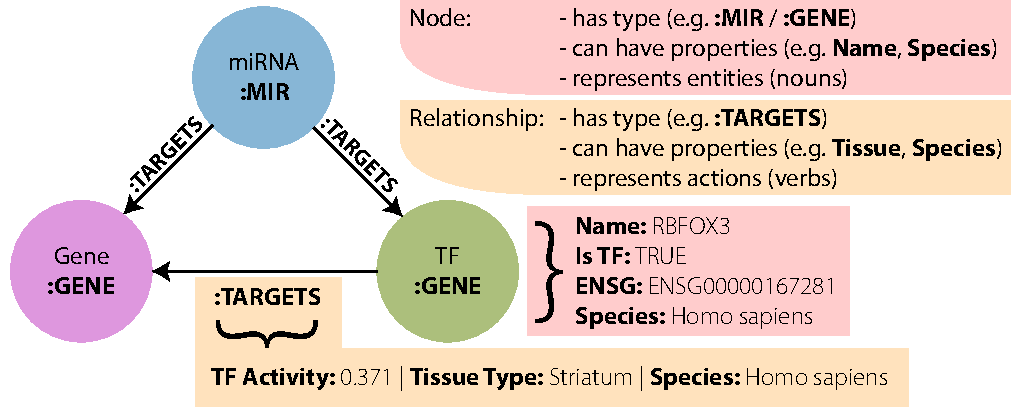
\includegraphics[width=\textwidth]{figures/graph-org}
\caption[Organisation of a Graph Database.]{\textbf{Organisation of a Graph Database.} A graph consists of two basic building blocks: \textit{Nodes}, representing entities, and \textit{edges}, representing connections between entities. Each database entry (node or edge) is an instance of a particular \textit{type} and can possess an arbitrary amount of \textit{properties} detailing its specifics.
\label{fig:graph-org}}
\end{figure}

Depending on the input, these queries can also be rather large; however, the main pitfall of tabular databases such as \ac{sql} is circumvented: there is no need to process entire rows or columns of the table to make sure that the query is satisfied in its entirety. This is particularly useful in a setting of sparse information. To illustrate: only 30 of the 2588 \acp{mir} target a specific gene, which is common; a relational database, after finding the index of the queried gene, would have to search 2588 fields for $1/0$. The graph database, on the other hand, has to execute only 30 searches (or, more accurately, 30 »walks« along the edges connected to the indexed node). In practice, even in the very first prototype implementations, this accelerated standard-case computations immensely, and was even able to accommodate advanced approaches in situations that had been inaccessible in the tabular implementation.

\subsection{High-throughput Database Generation}
Neo4j provides several \acs{api} (»application programming interface«) possibilities in implementation. For the purpose of entering large amounts of data into the database at once, the Java implementation is superior to the other forms in that it provides a batch processing mode via its \texttt{BatchInserter} class. I thus wrote a custom Java program for the purpose of creating an initial state of the database from the largest set of data, the complete miRWalk 2.0 content with 12 algorithms and validated interactions. The downloaded data was organised in a plain text based file format, with one text file for each \ac{mir}, totalling in size about 6 GB (for \textit{H. sapiens}). The database was set up in a way that allows only one node for each individual \ac{mir} and gene entered to avoid duplications, using the commands 
\begin{itemize}[noitemsep, leftmargin=.5cm, label={\tiny\raisebox{.5ex}{\textbullet}}]
\item \texttt{createDeferredConstraint()}
\item \texttt{assertPropertyIsUnique()}
\item \texttt{createDeferredSchemaIndex()} 
\end{itemize}
of the Neo4j Java package. This approach made sure to create only one node for each \ac{mir} (type: MIR) and gene (type: GENE) in the data, which is essential for proper functioning of the database. Each of these nodes received several properties to store individual data, such as the various gene/\ac{mir} identifiers, miRNA sequence, and species. 

Between those basic nodes, the batch insertion process created edges for each relationship that was found in the original data, assigning a type identifier to each edge detailing the origin of this interaction (type: name of the prediction algorithm or »VALIDATED« for experimental data). Thus, while the nodes for genes and \acp{mir} themselves are unique, an arbitrary number of relationships can exist between any two nodes, depending on how many interactions they share.

\subsection{Maintenance and Quality Control}
All additional datasets, such as the \ac{tf} regulatory circuits or \ac{trf} targeting predictions, were entered into \textit{miRNeo} using the regular operation mode. Testing was also performed in regular operation, with manual as well as automated tests to assert the correct transfer of information from raw data to the graph database, and to avoid unpredictable behaviour. At times, conflicts had to be resolved manually, for instance when \ac{mir} names conflicted between old »\ac{mir}*« and new »3p/5p« notation; all manual edits are documented in the code, which was published alongside Lobentanzer \emph{et al}.\cite{Lobentanzer2019a}

Except for the rapid import of large amounts of data in creation of a database, the Java implementation of Neo4j does not offer many advantages over the native R implementation, »RNeo4j«. Thus, after creation and a short period of experimentation with graphical user interfaces, I abandoned the Java program in favour of the more flexible R programming. While Java is an object-based programming language, whose benefits lie in extreme flexibility in regards to platform and purpose, high modularity, and speedy processing, R as a procedural language is the work horse of modern bioinformatics. Its procedural design (the division of data and functions that operate on that data) facilitates the transfer of approaches between distinct datasets, and the enormous vibrant community of data scientists using R provides a wealth of third party packages to tackle almost any bioinformatic task. In the remainder of this dissertation, all analyses are performed in R, unless specifically stated otherwise.

%%%%%%%%%%%%%%%%%%%%%%%%%%%%%%%%%%%%%%%%%%%%%%%%
%%%%%%%%%%%%%%%%%%%%% SECTION %%%%%%%%%%%%%%%%%%%%%
%%%%%%%%%%%%%%%%%%%%%%%%%%%%%%%%%%%%%%%%%%%%%%%%

\section{miRNeo - Materials}
All materials used in the creation of \textit{miRNeo} have been acquired from resources that are non\-/commercial, web-available, and open-source (in the case of code). All properties and relationships derived from this data were entered into \textit{miRNeo} as either nodes, properties of nodes, edges, or properties of edges. 

\subsection{Gene Annotation}
Even though »regular« protein coding genes have been known for a long time, there is no consensus yet about their nomenclature and organisation. Complicated by newly discovered functions and properties of phylogenetic nature, the scientific representation of the human genome is in constant flux. Several large organisations strive to provide a robust annotation of the human gene catalog, but also in many cases contradict one another. There are three nomenclature systems that are of high importance in modern genomics: 
\begin{itemize}[noitemsep, leftmargin=.5cm, label={\tiny\raisebox{.5ex}{\textbullet}}]
\item The traditional naming system of acronyms (e.g. \ac{chat}) and fantasy-names (such as »Sonic Hedgehog«), also occasionally called »gene symbol«, is still widely popular because of its accessibility to humans, but is also not particularly robust because of a high amount of synonyms with high confusion potential (see e.g. Section \ref{sec:intro:neurokine} on CDF) and instances of genes without names having to carry unwieldy systematic names. Gene symbols are largely, but not exclusively, curated by the HUGO Genome Nomenclature Consortium (HGNC), under the roof of the Human Genome Organisation (HUGO). As such, there also exists an »official« HGNC symbol for many genes, but these are not consistently used throughout the literature.
\item The American \ac{ncbi}, a branch of the National Institute of Health (NIH), curates and hosts a multitude of biological and medical data, and for the organisation of gene information uses its own systematic nomenclature termed »Entrez« ID. Entrez is a molecular biology database that integrates many aspects of biology and medicine in a gene-centred manner, and therefore Entrez IDs are useful to quickly connect a gene to its function, nucleotide sequence, or associated diseases. Entrez IDs are regular integers without additional characters.
\item Akin to the \ac{ncbi} effort, ENSEMBL is a project of the European Bioinformatics Institute (EBI) as part of the European Molecular Biology Laboratory (EMBL). Compared to the Entrez database, it is more focused on study and maintenance of the genome itself, and therefore has a more intricate nomenclature that allows for differentiation of, for example, genes and their various transcript isoforms (ENSEMBL IDs carry character prefixes for class identification, e.g., ENSG for genes, ENST for transcripts).
\end{itemize}
All of these are being used on a regular basis in many publications, and, often, they are used exclusively. As a result, the end user of the published data has to have access to all possible annotation forms, or, at least, a means to translate one into the other; often, this also introduces conflicts. For this reason, all ID types were entered into \textit{miRNeo} upon creation or during maintenance, for convenience and to minimise analysis prolongations due to conflict resolution.

\subsection{microRNA Annotation}
miRBase provides a consistent annotation for \acp{mir}. Due to their relatively recent discovery, there still are major changes from version to version; the syntax, however, is stable. In addition to the \ac{mir} »names« that are composed of species, the string »miR«, pre-\ac{mir} designation number, and strand origin (not in all cases!), such as »hsa-miR-125b-5p«, miRBase provides IDs for pre-\ac{mir} molecules (also called ancestors) termed »MIID«, and IDs for mature \ac{mir} molecules termed »MIMAT«. However, in practice, these are rarely used. Similarly, \ac{mir} families are annotated using the »MIPF« ID.

\subsection{Transcription Factor Targeting} \label{sec:database:tf}
The FANTOM5 project has applied \ac{cage} to a large number of human samples from diverse tissues to determine the accurate 5' ends of each transcript.\cite{Hon2017} Knowledge of this fact enables accurate prediction of transcription factor binding sites likely to control a transcript's expression. Marbach and colleagues used this information in combination with detailed human gene expression data to derive a complex interaction network of \acp{tf} and genes (»regulatory circuits«), and in doing so aggregated samples with similar expression patterns and origins into 394 fictional tissues.\cite{Marbach2016} For every tissue, each \ac{tf} was assigned transcriptional activities towards all genes that it supposedly targets (with the sum of all activities in any given tissue being \num{1}). Marbach and colleagues have shown that the cumulative transcriptional activities towards any given gene correlate well with the actual gene expression in corresponding samples from an independent repository.

Even in its fifth iteration, FANTOM data is not entirely comprehensive, which came to my attention due to a cholinergic anomaly: The 5' \ac{cage} peaks of the \textit{\ac{chat}} and \textit{\acs{a7}} (the nicotinic $\alpha$7 receptor subunit) genes in raw FANTOM5 brain tissue data do not pass the expression threshold, and therefore are not included in, e.g., Marbach's »regulatory circuits«. Both are critically important not only for neuronal cholinergic systems, but also for the non-neuronal aspect of immune processes. For instance, macrophages have been shown to produce \ac{ach} via \ac{chatp}, and the $\alpha$7 homomeric \ac{ach} receptor conveys direct immune suppression by its expression on monocytes.\cite{Fujii2017} Paradoxically, the \ac{cage} peak of \textit{\ac{slc}}, which lies in the first intron of \textit{\ac{chat}}, crosses the threshold and therefore is included in the data. Unfortunately, I was not able to remedy these circumstances even upon personal communication with Daniel Marbach (author of »regulatory circuits«) and Hideya Kawaji of the FANTOM5 consortium, although the latter acknowledged the possibility of a gene annotation deficit leading to misattribution of the \textit{\ac{chat}} signal to \textit{\ac{slc}} due to the closeness of their 5' ends. Thus, it seems viable to substitute \emph{SLC18A3} targeting data for the absent \emph{CHAT} data in certain situations.

The entire collection of transcriptional activities in all tissues was downloaded from the project's web page,\cite{Marbach2016} and neuronal and immune tissues were manually curated and entered into \textit{miRNeo}. The collected data comprises 33 neuronal tissues and 26 immune cell tissues (Appendix \ref{appendix:marbach}), and \num{1130196} \ac{tf}$\to$gene relationships in total (not all 394 tissues were entered due to the time requirements). 

\subsection{microRNA Interactions} \label{sec:database:mirna}
The content of miRWalk 2.0 is freely available online;\cite{miRWalk2} however, there is no option of downloading the complete set. The targeting data thus was downloaded per \ac{mir} using a custom crawler, with standard options for all 12 prediction algorithms (miRWalk, miRDB, PITA, MicroT4, miRMap, RNA22, miRanda, miRNAMap, RNAhybrid, miRBridge, PICTAR2, and TargetScan) in plain text format. For experimentally validated interactions, the main sources were DIANA TarBase\cite{Karagkouni2018} and miRTarBase,\cite{Chou2018} both of which offer complete download options. As of 2019, the 3.0 version of miRWalk allows complete species downloads; however, the developers have abandoned their third party algorithm plurality reducing the number of available alternatives from 12 to 4, which can be considered a significant disadvantage:

While sequence complementarity, particularly of the »seed«-region, is the primary paradigm of \ac{mir}-mRNA interaction, prediction algorithms vary widely in their implementation, general purpose, and approach to interaction prediction (for a comprehensive review of approaches and rules, see Yue \emph{et al.}\cite{Yue2009}). A large group of available options utilise sequence conservation aspects to increase candidate viability (such as miRanda, PicTar, TargetScan, and microT4). Others, such as RNA22 and PITA, utilise biophysical aspects such as free energy of binding or the accessibility of target sites due to secondary RNA structures as prediction arguments. All of these approaches have their up- and downsides, e.g. considering their general precision and sensitivity, or their adequate prediction of particular cases, such as multiple site targeting. Thus, it has been proposed to use a combination of complementary approaches instead of only one algorithm per analysis.\cite{Witkos2011} For this reason, I may have preferred the 2.0 version of miRWalk, even if 3.0 had been available at the time.

One advantage of the collection of all data in a quickly accessible database is the opportunity to compare the different approaches to target prediction. A statistical evaluation of the collected interaction data from miRWalk 2.0 showed vast differences in general prediction quantity (Table \ref{tab:alg.hit.freq.all}) as well as prediction accuracy and sensitivity when compared to the validated subset of data (Table \ref{tab:alg.hit.freq.val}). Since the ground truth is not known, this is an additional argument for the combination of multiple algorithms instead of the use of a single set. Apart from RNAhybrid and miRBridge, all algorithms presented reasonable base hit frequencies and increases in the validated test set. While miRBridge already has the lowest positive frequency of all the algorithms, it is the only one to achieve a negative score in the validated test set. On the other hand, RNAhybrid has a vastly higher base hit frequency than the second highest scoring algorithm (by more than \num{300}\%), making it very likely to produce false positive results, and less valuable in the aggregation scoring system. The remaining 10 algorithms were included in \textit{miRNeo} targeting data. For ease of use, an additional relationship type was created from the aggregated single algorithm hits of any \ac{mir}$\to$gene relationship, with the sum of algorithms predicting the interaction as a score variable. This yields a theoretical score range from \num{3} to \num{10} (\ac{mir}$\to$gene relationships with only one or two hits were ignored for the sake of space). To account for experimentally validated interactions, each \ac{mir}$\to$gene relationship that was supported by strong evidence of interaction was modified by addition of \num{10.5} score points (a half point for quick identification of a validated relationship), extending the maximum score to \num{20.5} points. The resulting optimised graph contains \num{11687931} human \ac{mir}$\to$gene targeting relationships with a distinct score distribution (Fig.\,\ref{fig:db-score-hist}). In comparison, only 6146 \ac{mir}$\to$gene relationships are experimentally validated with »strong« evidence.

\begin{figure}
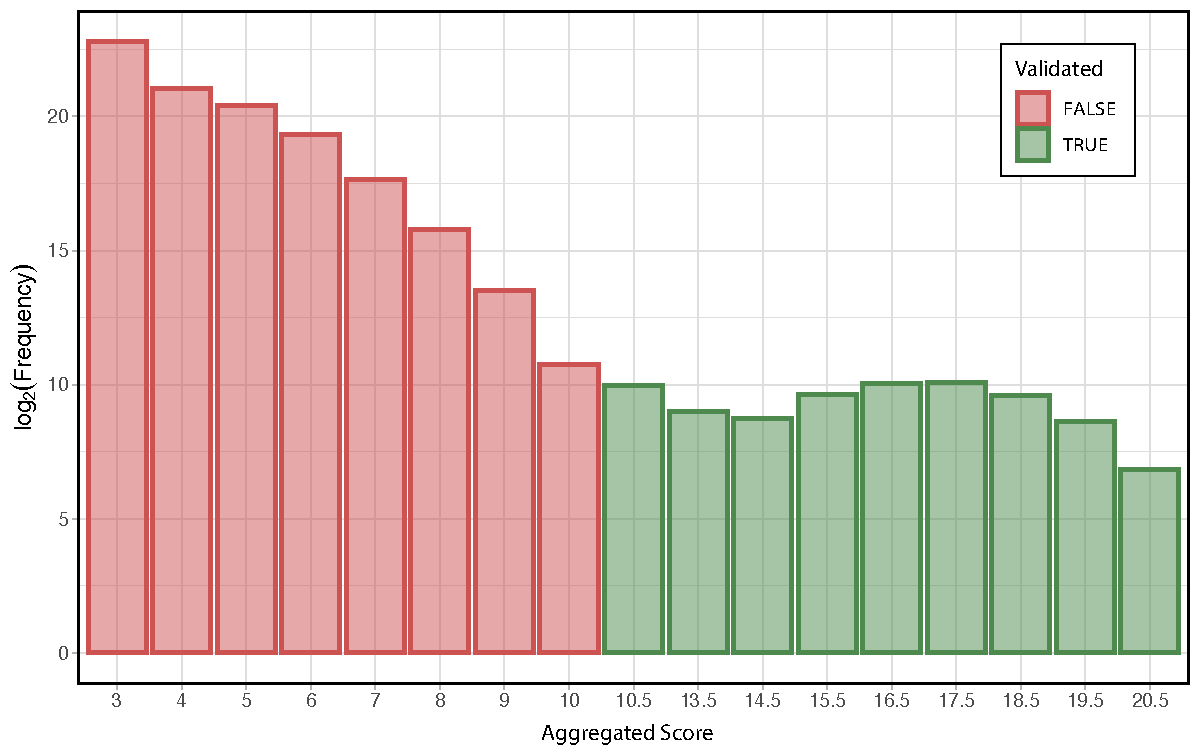
\includegraphics[width=\textwidth]{figures/db-score-hist}
\caption[Histogram of \ac{mir}$\to$Gene Score Distribution.]{\textbf{Histogram of \ac{mir}$\to$Gene Score Distribution.} Aggregation of individual algorithms yields a score range of 3 to 10 per individual \ac{mir}$\to$gene interaction. In case of additional existence of experimental validation (evidence level high) for any predicted interaction, score is increased by 10.5. The distribution shows a sharp decrease in predicted interactions towards higher scores, and a maximum of validated interactions at prediction scores 6 and 7. 
\label{fig:db-score-hist}}
\end{figure}

%tables from cholinomir pseudopaper
\begin{table}
\sffamily
\small
%\resizebox{.85\textwidth}{!}{%
\noindent\parbox[t]{.35\linewidth}{
\centering
\begin{tabular}{c | c}
algorithm & hit frequency\\ \hline
\hline
\textcolor{Maroon}{RNAHYBRID} & 71.62\%\\ \hline
\textcolor{OliveGreen}{MIRMAP} & 19.90\%\\ \hline
\textcolor{OliveGreen}{MIRWALK} & 19.74\%\\ \hline
\textcolor{OliveGreen}{TARGETSCAN} & 16.33\%\\ \hline
\textcolor{OliveGreen}{RNA22} & 12.34\%\\ \hline
\textcolor{OliveGreen}{MICROT4} & 11.81\%\\ \hline
\textcolor{OliveGreen}{MIRANDA} & 10.65\%\\ \hline
\textcolor{OliveGreen}{PITA} & 4.90\%\\ \hline
\textcolor{OliveGreen}{MIRDB} & 1.17\%\\ \hline
\textcolor{OliveGreen}{MIRNAMAP} & 0.75\%\\ \hline
\textcolor{OliveGreen}{PICTAR2} & 0.62\%\\ \hline
\textcolor{Maroon}{MIRBRIDGE} & 0.15\%\\ \hline
\end{tabular}
\caption{Prediction algorithms ordered by the fraction of all possible interactions they predict as being real (positive rate). Different algorithms display a wide variation of hit rates in the entirety of predicted interactions between any \ac{mir} and gene. Red: excluded from analysis.}
\label{tab:alg.hit.freq.all}
}
\hfill
\noindent\parbox[t]{.6\linewidth}{
\begin{tabular}{c | c | c}
algorithm & validated hit frequency & hit rate increase\\ \hline
\hline
\textcolor{OliveGreen}{PICTAR2} & 6.98\% & 1129.40\%\\ \hline
\textcolor{OliveGreen}{MIRDB} & 9.80\% & 838.43\%\\ \hline
\textcolor{OliveGreen}{MIRANDA} & 51.73\% & 485.94\%\\ \hline
\textcolor{OliveGreen}{TARGETSCAN} & 70.63\% & 432.51\%\\ \hline
\textcolor{OliveGreen}{MIRNAMAP} & 3.10\% & 410.95\%\\ \hline
\textcolor{OliveGreen}{PITA} & 15.57\% & 317.20\%\\ \hline
\textcolor{OliveGreen}{MICROT4} & 32.60\% & 276.10\%\\ \hline
\textcolor{OliveGreen}{MIRMAP} & 53.86\% & 270.65\%\\ \hline
\textcolor{OliveGreen}{MIRWALK} & 50.95\% & 258.15\%\\ \hline
\textcolor{OliveGreen}{RNA22} & 22.51\% & 182.38\%\\ \hline
\textcolor{Maroon}{RNAHYBRID} & 90.47\% & 126.32\%\\ \hline
\textcolor{Maroon}{MIRBRIDGE} & 0.01\% & 0.00\%\\ \hline
\end{tabular}
\caption{Prediction algorithms ordered by their increase in true positive rate when considering only validated interactions. The hit rate increase when comparing experimentally validated interactions with the entire predicted data (Table \ref{tab:alg.hit.freq.all}) is also subject to strong variation. Hit rate increase is the increase of hit rate if only considering validated data as opposed to all predicted interactions. None of the studied algorithms unite a good precision (hit rate increase) and coverage (validated hit frequency).}
\label{tab:alg.hit.freq.val}
%}
}
\end{table}

\subsection{Filtering of Aggregated Prediction Scores}
For the estimation of the »true« \ac{mir}$\to$gene interactions in the predicted-only data in \textit{miRNeo}, two premises are relevant: First, the enormous amount of hits with a score of 3 in all likelihood is an over-estimation, and second, the amount of currently validated interactions can be but a small fraction of »true« interactions. Assuming the truth lies on the axis between these two extremes (i.e., at some score value inside the \textit{miRNeo} interactions), the true amount of human \ac{mir}$\to$gene interactions must approximately fall within the range of $2^{10}$ to $2^{20}$. Looking at the score distribution of all \textit{miRNeo} interactions (Fig.\,\ref{fig:db-score-hist}), the maximum amount of validated interactions is predicted by a combination of 6 or 7 algorithms (i.e., a score of 16.5 or 17.5). Thus, to approximate the true state, I chose to apply a low-cut filter to \textit{miRNeo} queries at a minimum score of 6. This is the standard case referred to as »\textit{miRNeo} query« in the remainder of this dissertation. In some cases, such as the graphical analysis of whole-genome \ac{mir} targeting (see e.g. Section \ref{sec:cellculture:network}), the score threshold was raised to 7 to circumvent computational limitations.

\subsection{De-novo Prediction of tRF Targeting} \label{sec:database:trf-targeting}
Due to the recency of their (re-)discovery, no comprehensive interaction sources exist for \acfp{trf}. There have been documented cases of \ac{mir}-like behaviours of distinct RNA fragments,\cite{Cole2009,Kumar2014} justifying an attempt to predict interactions in a comprehensive manner. Of the available options for nucleotide interaction prediction algorithms, TargetScan\cite{Friedman2009} seems particularly suited for this task because it provides the option of evaluating the evolutionary conservation of target sites in the putatively targeted genes, thereby providing an additional layer of security: The sequence of 3' \acp{utr} is evolutionarily less stable than the coding part of genes; thus, high conservation of the binding site may indicate evolutionary pressure to keep up the interaction with the fragment, making an actual function of the interaction more likely. TargetScan also presents with reasonable sensitivity and specificity as confirmed by an independent group,\cite{Alexiou2009} and through an additional algorithm allows the attribution of a score based on the branch length (on the species tree) of conserved targeting.\cite{Agarwal2015}

\ac{mir}-like behaviour implies the existence of a region on the \ac{trf} similar to a \ac{mir} »seed«, and TargetScan also expects a seed as input to its targeting algorithm. Since there has been no definitive answer to the question as to where the seed region in \acp{trf} may be, it is safest to assume nothing and explore all possibilities, i.e., simulate every possible seed position for interaction discovery. For this purpose, all discovered sequences of \acp{trf} (exceeding a base mean expression of 10 counts) were chopped into 7-nt pieces (7mers), which is the length of \ac{mir} seeds, and statistically improbable enough to appear in the genome at random; the average length of a human 3' \ac{utr} is 800 \ac{nt}, so the probability of finding any 7mer randomly in any one 3' \ac{utr} is $p = \frac{800}{4^7} = 0.049$, which agrees with the 5\% \ac{fdr} convention.

\subsection{microRNA Primate Specificity}
During the course of evolution, higher organisms typically attained more complexity in a variety of functional categories. The \ac{cns} as the system of highest complexity underwent several drastic developments from invertebrates to lower mammals to higher mammals still. miRNAs are no exception. While many miRNAs are functionally as well as literally conserved in all mammals, primates in particular have gained a substantial amount of novel miRNAs whose function is in large parts elusive. Due to the restrictions on experimentation on higher mammals, particularly primates, many of those miRNAs can only be studied observationally, or by transgenic experiments in rodents. A cholinergic example of a gain-of-function in higher mammalian miRNA regulation is the vesicular acetylcholine transporter, \ac{slc}. As described in Section \ref{sec:database:tf}, the \ac{slc} gene is situated in the first intron of \ac{chat}, and thus is always primarily co-expressed with the latter. However, a primate-specific miRNA, miR-298, targets the 3' UTR of \ac{slc}.\cite{Soreq2015} Thus, the primate neuron has gained a mechanism of independent \ac{slc}/\ac{chat} regulation that the mouse, for example, does not possess. It is easily imagined that such a gain of neuronal flexibility, in many instances, can aid the development of a more effective brain. However, the primate specificity of miRNAs is not yet consensus, and thus not found in annotation databases such as miRBase, even though they list all miRNAs discovered in any species. To get an impression of the amount of possible gain of function, I performed a review of miRNAs expressed in a representative variety of annotated species. From hereon out, largely method-related paragraphs will be set in sans-serif font face.

\begin{method}

\subsubsection{Species Selection}
The tested species were selected from miRBase v21. Some of the available species are severely limited in the extent of miRNA annotation, likely because of a research bias. Therefore, only the most well-annotated species were selected. These are (number of annotated primary and mature miRNAs in brackets):
\begin{itemize}[noitemsep, leftmargin=.5cm, label={\tiny\raisebox{.5ex}{\textbullet}}]
\item \emph{Homo sapiens} (human; 1881, 2588)
\item \emph{Gorilla gorilla} (gorilla; 352, 357)
\item \emph{Pan troglodytes} (chimp; 655, 587)
\item \emph{Pongo pygmaeus} (orangutan; 642, 660)
\item \emph{Macaca mulatta} (rhesus macaque; 619, 914)
\item \emph{Bos taurus} (cow; 808, 793)
\item \emph{Canis familiaris} (dog; 502, 435)
\item \emph{Mus musculus} (mouse; 1193, 1915)
\item \emph{Rattus norvegicus} (rat; 495, 765)
\end{itemize}
The first four species belong to the hominid group; the first five are primates. It is likely that these collections are not complete, with the degree of completeness depending on the amount of research performed on the species (as demonstrated, e.g., by the difference between mouse and the other non-primates). This places considerable difficulty on asserting primate specificity of miRNA, and in turn on assertion of the effects of evolution on the miRNA regulatory system.

\subsubsection{Single miRNA Inter-Species Homology Computation}
To determine the homology of miRNAs between the studied species, reference genomes were downloaded from the respective sources and analysed phylogenically, using the genomic coordinates provided by miRBase. Homology of sequences was determined via dynamic programming using the Smith-Waterman algorithm.\cite{Smith1981} Briefly, this algorithm can be used to determine the similarity of two genomic sequences, based on a scoring system rewarding matches and penalising mismatches. Smith and Waterman extended the original approach by Needleman and Wunsch,\cite{Needleman1970} which is used to compare two complete sequences. Both algorithms rate an alignment by dynamic scoring inside a 2D-matrix, with the sequences to be compared as the x- and y-axes (one letter per cell). By a change in the scoring system, the Smith-Waterman algorithm finds the best local alignments, instead of comparing the two sequences in their entirety. In the case of miRNAs, this behaviour is useful because, between species, there are frequent additions or deletions of single \ac{nt} on both ends of the homologous miRNA. Genomes were procured from the following sources:
\begin{itemize}[noitemsep, leftmargin=.5cm, label={\tiny\raisebox{.5ex}{\textbullet}}]
\item \emph{Homo sapiens}: GRCh38 (NCBI)
\item \emph{Gorilla gorilla}: gorGor3 (UCSC)
\item \emph{Pan troglodytes}: panTro4 (UCSC)
\item \emph{Pongo pygmaeus}: PPYG2 (Ensembl)
\item \emph{Macaca mulatta}: rheMac3 (UCSC)
\item \emph{Bos taurus}: bosTau6 (UCSC)
\item \emph{Canis familiaris}: canFam3 (UCSC)
\item \emph{Mus musculus}: mm10 (UCSC)
\item \emph{Rattus norvegicus}: rn5 (UCSC)
\end{itemize}

Using the genome coordinates provided by miRBase, the genomic sequences of miRNAs and pre-miRNAs of each species were determined. Using the Smith-Waterman algorithm, all identified homologs of human miRNAs were subjected to homology scoring, and score results were visualised as a heatmap.

\end{method}

\subsubsection{Inter-Species Distribution of miRNAs}
The inter-species relationships of annotated miRNAs do not follow a simple evolutionary distribution from less complex to more complex organisms, but rather seem to partially result from parallel development (Fig. \ref{fig:species-homo}). Taking into account the high probability of missing annotations in several species (particularly hominids), it seems prudent to define primate specificity of miRNAs not by presence in primates, but rather by absence of the miRNAs in non-primate species (also excluding miRNAs \emph{only} annotated in human). Thus, primate specificity of a human miRNA is assumed if the miRNA is expressed in at least one primate species, and absent from all non-primate species in this roster. This definition yields a list of 377 primary and 350 mature putative “primate specific” miRNAs in miRBase v21 (Appendix \ref{appendix:homologues}). Judging from recent analyses,\cite{Londin2015} there probably exist many more. The primate-specificity attribute was entered into \emph{miRNeo} as miRNA node property.

\begin{figure}
\centering
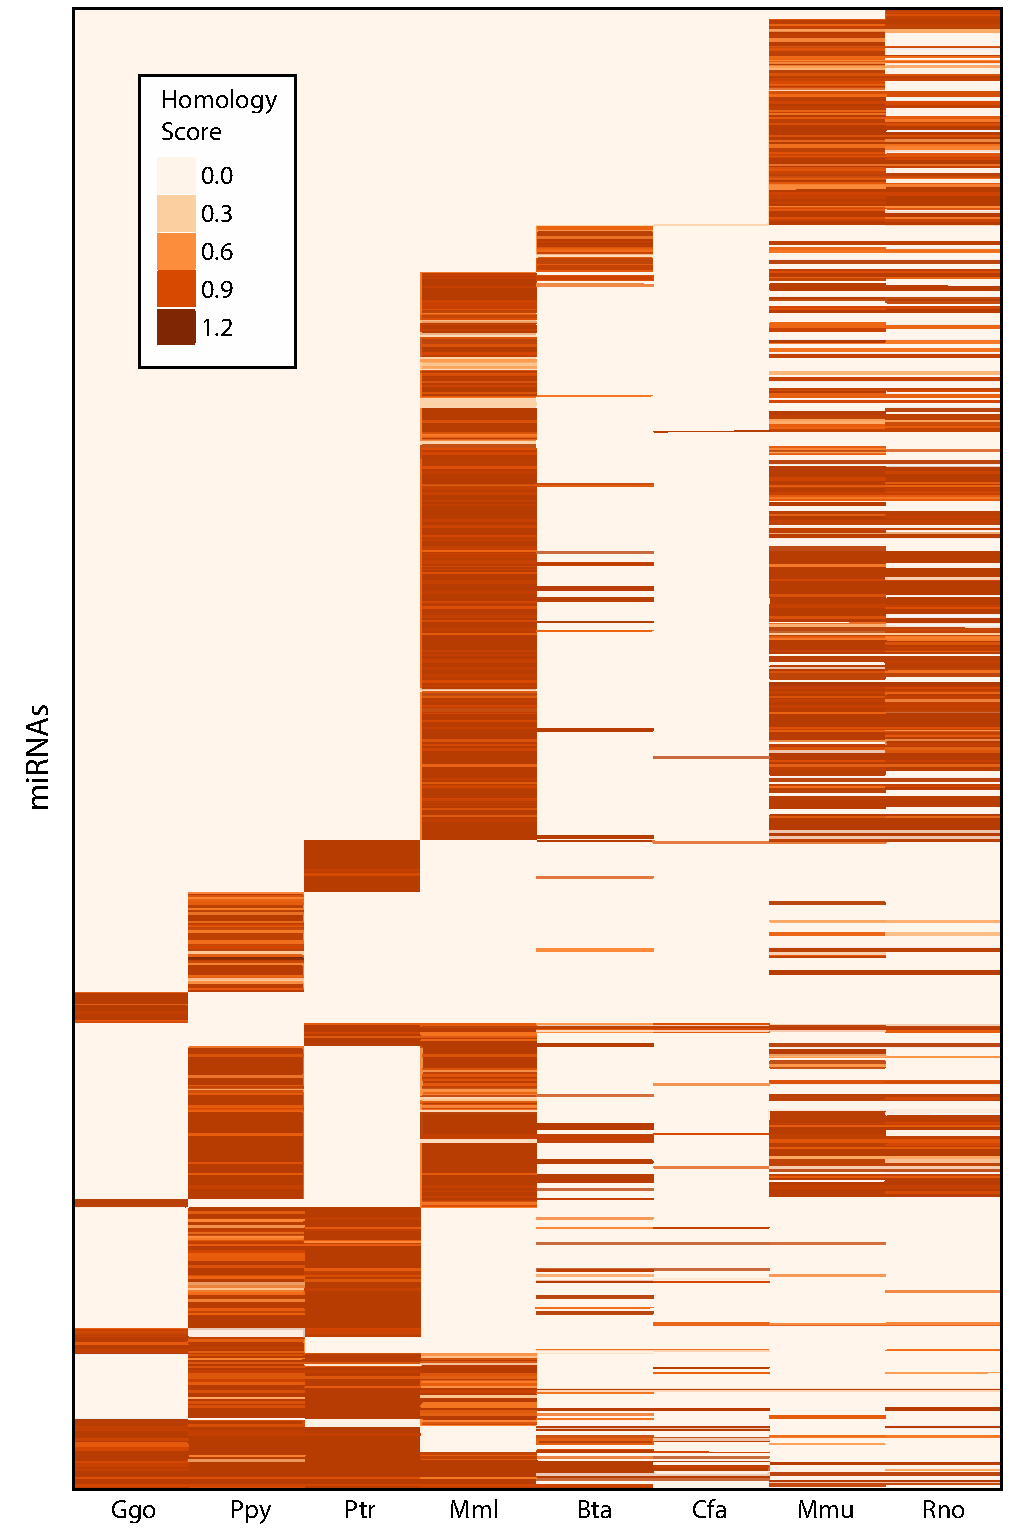
\includegraphics[width=.9\textwidth]{figures/species-homo}
\caption[microRNA Species Homology.]{\textbf{Homologues of Human microRNAs in Primate- and Non-Primate-Species.} Homology to human miRNAs was determined by Smith-Waterman local alignment for each homologous miRNA of 8 species. Homology scores were visualised on a heatmap, each column represents the homology to human of the miRNAs of the respective species. The heatmap is ordered from bottom to top by the amount of miRNA homologues in primates. The miRNAs at the very bottom are shared by human as well as all four primate species, followed by the miRNAs shared by three primate species, and so on. Ggo: \emph{Gorilla gorilla}, Ppy: \emph{Pongo pygmaeus} (Orangutan), Ptr: \emph{Pan troglodytes} (Chimp), Mmt: \emph{Macaca mulatta} (Rhesus macaque), Bta: \emph{Bos taurus} (Cow), Cfa: \emph{Canis familaris} (Dog), Mmu: \emph{Mus musculus} (Mouse), Rno: \emph{Rattus norvegicus} (Rat).
\label{fig:species-homo}}
\end{figure}

%%%%%%%%%%%%%%%%%%%%%%%%%%%%%%%%%%%%%%%%%%%%%%%%
%%%%%%%%%%%%%%%%%%%%% SECTION %%%%%%%%%%%%%%%%%%%%%
%%%%%%%%%%%%%%%%%%%%%%%%%%%%%%%%%%%%%%%%%%%%%%%%

\section{miRNeo - Usage} \label{sec:database:usage}
Neo4j uses a language (called »Cypher«) akin to \ac{sql}, which utilises keyphrases to issue commands, but combines it with a semi-graphical syntax to account for the graph-based layout of the data. In the following, I will describe its basic usage and the advantages it provides in the matter of transcriptional connectomics. The basic »finder« function (similar to \textcolor{dkblue}{SELECT} in \ac{sql}) is called \textcolor{dkblue}{MATCH} in Cypher, and, when combined with the semi-graphical syntax, can be used to identify nodes or more complex patterns in the database. The graphical syntax consists of two main building blocks that represent the basic types of data inside the database: nodes as regular brackets »\textbf{\texttt{( )}}« and edges between nodes as  a construct of hyphens and box brackets, that can also have a direction indicated by the greater sign \mbox{»\textbf{\texttt{( )-\string[ \string]->( )}}«}. To specify the elements to be found, attributes of nodes and/or edges can be filtered by using curly brackets in the node definition, or the \textcolor{dkblue}{WHERE} clause. To be returned, elements need to be assigned arbitrary variable names:

\begin{lstlisting}[label=lst:match, caption=MATCH, language=Cypher]
MATCH (gene:GENE {species: 'HSA'})
WHERE gene.name = 'CHAT'
RETURN gene
\end{lstlisting}

Query \ref{lst:match} identifies a node (arbitrarily designated »gene«) with type GENE (indicated by the colon), with attributes »species« (HSA, i.e. \textit{H. sapiens}) and »name« (\ac{chat}), and returns the node with all its attributes. Since the nodes of type GENE are restrained, there can only be one gene of species \textit{H. sapiens} with this name in the database, and thus, only one data point will be returned. The graphical syntax further allows for pattern matching of, for instance, \ac{mir}$\to$gene relationships:

\begin{lstlisting}[label=lst:pattern,caption=Patterns,
language=Cypher]
MATCH (mir:MIR)-[rel:TARGETS]->(gene:GENE {species: 'HSA'})
WHERE gene.name = 'CHAT'
RETURN mir, rel, gene
\end{lstlisting}

Query \ref{lst:pattern}, similar to query \ref{lst:match}, starts by identifying the node of species HSA with the name \ac{chat}, and proceeds to look for \ac{mir}$\to$gene relationship edges arriving at this node; the relationships have to be of the type TARGETS (the pre-aggregated score-based accumulation of targeting). As soon as no further edges are found, the process terminates and returns all found \acp{mir} (»mir«), relationships (»rel«), and genes (»gene«) in discrete form, including all their attributes, such as the ENSG and Entrez IDs, the MIMAT IDs for all found \acp{mir}, or the score value of their targeting relationship. In this query, since there is a constraint on genes, the only gene returned is \textit{\ac{chat}}. However, Cypher is not limited to filtering on unique attributes; it allows for query and return of as many data points as are needed. For example, if one is interested in all \ac{mir}$\to$gene interactions in the cholinergic system, the query may look as follows:

\begin{lstlisting}[label=lst:filter,caption=Filtering,
language=Cypher]
MATCH (mir:MIR)-[rel:TARGETS]->(gene:GENE {species: 'HSA'})
WHERE gene.name IN {cholinergic_genes}
RETURN mir, rel, gene
\end{lstlisting}

The effectiveness of graph-based databases becomes clear in this approach: Query \ref{lst:filter} is processed starting at a user-defined filter, the list of cholinergic genes as an input (containing \textit{\ac{chat}}, \textit{\ac{slc}}, cholinergic receptor genes, \acl{ache}, etc). In a first step, all nodes are found that fulfil the criteria: type GENE, from species \textit{H. sapiens}, that are in the list of names given. Since the gene nodes are indexed, this only requires milliseconds. Then, through the connection of edges to these nodes, it finds all \ac{mir} nodes that have a \ac{mir}$\to$gene relationship towards any of the cholinergic genes. By using the gene nodes as starting point, the query can end as soon as no other edges fulfilling these criteria are found on any of the nodes. In comparison, to satisfy this query in a relational database, the rows representing these cholinergic genes would have to be assessed in their entirety, not only in those columns that represent an extant relationship, thus prolonging execution.

The database then returns all \ac{mir}$\to$gene relationships in this set, representing the network of cholinergic \ac{mir} regulators, including all of their attributes. The advantages of graph-based data do not end there; say one wants to return only »master« regulators of cholinergic systems, defined as \acp{mir} that target at least 4 of the genes in the cholinergic set. In a relational database, this would have to be done post-hoc, by aggregation of relationships and removal of any results that do not exceed this threshold. This requires storage of the entire result in memory, and additional computational steps that can be very taxing depending on the size of the result table. In Cypher, this can be done during the query (code comments indicated by »\textcolor{dkgreen}{//}« explain single steps):

\pagebreak

\begin{lstlisting}[label=lst:filter2,caption=Two-stage Filtering,
language=Cypher]
MATCH (gene:GENE {species: 'HSA'})
WHERE gene.name IN {cholinergic_genes}
WITH gene //the found genes are used as input for the second query
MATCH (mir:MIR)-[rel:TARGETS]->(gene)
WHERE count(rel) >= 4
RETURN mir, rel, gene
\end{lstlisting}

Query \ref{lst:filter2} essentially proceeds in the same way as query \ref{lst:filter} in that it identifies the gene nodes filtered for and looks for the \acp{mir} connected to those nodes by TARGETS-type relationships; however, in the second step (which is performed per gene node as returned by the \textcolor{dkblue}{WITH} clause), it returns only those patterns that have at least 4 incoming \ac{mir}$\to$gene relationships. Query \ref{lst:filter2} only requires little additional processing compared to query \ref{lst:filter}, and thus does not require nearly as much time as the post-hoc filtering required in a relational database query. This filtering can be applied in many stages, and in many forms, such as sums, averages, maximum and minimum, or other combinations of arithmetic and logical classifiers. Additionally, the patterns can be extended to represent complex relationships inside the graph. For instance, the following query \ref{lst:loop} was used to find \acp{mir} that regulate any given gene in the database, and, simultaneously, affect \acp{tf} that are involved in regulation of this same gene (this type of interaction is called feedforward loop, see also Section \ref{sec:stroke:ffl}).

\begin{lstlisting}[label=lst:loop,
caption=Feedforward Loop Identification,
language=Cypher]
MATCH (gene:GENE) //find gene
WHERE gene.id = ID //by identifier (Entrez)
WITH gene //use as input for next step
MATCH (tf:GENE {species: 'HSA', tf:TRUE})-[rel]->(gene) 
//find TFs targeting that gene
WHERE type(rel) IN {tissue_types} //TFs only from specific tissues
//for instance, CNS cell types (Appendix A)
WITH gene, rel, tf //use as input for next step
MATCH (tf)-[rel]->(gene)<-[rel_m1:TARGETS]-(mir:MIR {species: 'HSA'})-[rel_m2:TARGETS]->(tf) 
//find miRNAs that target gene and gene-targeting TF at the same time
WHERE rel_m1.score > 5 AND rel_m2.score > 5 
//low-cut filter at a minimum cumulative score of 6
RETURN gene, tf, rel, type(rel) AS tissue, mir, rel_m1, rel_m2
\end{lstlisting}

This analysis can be performed in real time, on the whole genome and miRnome, and merely takes seconds for one iteration, a performance unimaginable in a relational database approach; advanced statistical approaches such as permutation only become viable at this timescale.

%%%%%%%%%%%%%%%%%%%%%%%%%%%%%%%%%%%%%%%%%%%%%%%%
%%%%%%%%%%%%%%%%%%%%% SECTION %%%%%%%%%%%%%%%%%%%%%
%%%%%%%%%%%%%%%%%%%%%%%%%%%%%%%%%%%%%%%%%%%%%%%%

\section{Statistical Approach to Transcriptional Connectomics}
The enormous amounts of data generated by modern molecular biology methods, such as \ac{seq} and bioinformatics, present new challenges to statistical methodology. A major objective in the analysis of large datasets is a robust statistical representation of the distribution of this data. Traditionally used approaches such as Student's t-test are not automatically applicable to the intermediary results of these modern methods, because the premise of a normal distribution often does not hold, or has to be proven first. This section will describe the statistical problems encountered in the analysis of intermediary data produced by \textit{miRNeo}; the statistical properties of large count data directly generated by \ac{seq} will be discussed in Sections \ref{sec:cellculture:deseq} and \ref{sec:discussion:rna-seq}.

\begin{method}

\subsection{Permutation} \label{sec:database:permutation}
The evaluation of comprehensive prediction datasets regarding \ac{mir}$\to$gene interactions on a genome scale is statistically challenging. Molecular interaction studies have explored only a minority of all possible targeting relationships, and as such, the ground truth of \ac{mir}$\to$gene interaction is unknown (see Section \ref{sec:database:mirna}). Since there is no negative interaction data, validated interactions can only be defined in the positive space. Additionally, the various prediction algorithms also heavily diverge in their predictions, which leads to the question of how to approach the estimation of \acf{fdr} while simultaneously avoiding high false negative rates.

One possible approach that can aid in identification of the most pertinent effects in this case is random permutation. In this approach, the result of an analysis (e.g., a numeric targeting score of a \ac{mir}$\to$gene interaction, or a Spearman correlation between two gene sets) is compared to a null distribution that was generated from an iterative analysis similar to the initial one, but with randomised input (e.g., a group of \acp{mir} of the same size as the original set, randomly selected from all \acp{mir}, or the gene sets from the original analysis with randomly scrambled group affiliations). This permutation of the analysis is performed many times (usually between \num{10000} and \num{1000000} iterations, depending on the context), and results in a distribution of possible outcomes that can be arranged from lowest to highest, often resulting in a normal (or »normal-like«) distribution, thus facilitating the estimation of confidence intervals, and, similarly, p-values for the »real« result.

A positive side-effect of performing a permutation analysis on a base collection of data, such as \textit{miRNeo}, is the automatic correction of inherent biases. For instance, should a particular gene by its genetic structure invite a large amount of false positive predictions as to the \ac{mir}$\to$gene interactions towards it, these will be present in the test as well as in the permutation comparison, and thus cancel out and yield a high p-value for this interaction, effectively transforming the false positive into a true negative. For further discussion, see Section \ref{sec:discussion:network-statistics}.

\subsection{Gene Set Enrichment Analysis} \label{sec:database:gsea}
The objective of gene set enrichment is the identification of statistically over-represented entities in a dataset. The standard use case in biomedicine is the Gene Set Enrichment Analysis (GSEA), that is used to identify the most important classes of genes in large datasets, such as the ones produced by \ac{seq}. Briefly, the analysis follows these steps: the studied genes are scored by a certain method, such as p-values from differential expression analysis, which enables the identification of a relevant subgroup, the test set (e.g., the 100 genes with lowest p-values). This test set is then compared to a background of genes (usually, all detected genes, or a large amount of genes from the entire dataset) by a statistical method fit to determine their enrichment in pre-defined categories. Often, ontological categories are used, such as the »biological process« type of \ac{go}, or KEGG pathways.

For each of these categories, the method tests for a representation of genes in the test set exceeding the frequency statistically expected by random sampling from the background of genes; thus enabling an estimation of the functionality these test set genes may inhabit in the process that is studied. Statistical approaches often employed in gene set enrichment are Kolmogorov-Smirnov statistics, permutations, or, more generally, hypergeometric tests such as Fisher's exact test. There are a wide variety of software solutions available for the implementation of gene set enrichment testing.

\acl{go} curates an enormous catalogue of coding gene products and their functions. At the current time, \ac{go} hosts \num{7330378} annotations (\num{2836377} for »biological process«, \num{2289165} for »molecular function«, and \num{2204836} for »cellular component«), subdividing \num{1405197} individual gene products from \num{4493} species (\num{205} with more than \num{1000} annotations) into \num{44733} ontological terms (\num{29457} »biological process«, \num{11093} »molecular function«, and \num{4183} »cellular component« terms). The individual GO categories are organised in a hierarchical manner, more specifically, a \ac{dag}. Each branch of the DAG tree contains related terms, progressing from the most general terms (top) to the most specific ones (at the bottom). 

Whenever a \ac{go} analysis is described in chapters three and four, it means a gene set enrichment analysis performed on a particular subset of genes (that may e.g. be the targets of a group of \acp{mir}) towards the elucidation of their biological function, i.e., the »biological process« category of \ac{go} annotation. For further discussion, see Section \ref{sec:discussion:go}.

\end{method}

%!TEX root = ../dissertation.tex
\begin{savequote}[60mm]
There is no scientific study more vital to man than the study of his own brain. Our entire view of the universe depends on it.\qauthor{Francis Crick}
\end{savequote}

% If the human brain were so simple that we could understand it, we would be so simple that we couldn’t.
% – Emerson M. Pugh

% The human brain, then, is the most complicated organization of matter that we know.     
% Isaac Asimov

% One of the difficulties in understanding the brain is that it is like nothing so much as a lump of porridge.
% Richard L. Gregory

% The brain is a monstrous, beautiful mess. Its billions of nerve cells - called neurons - lie in a tangled web that displays cognitive powers far exceeding any of the silicon machines we have built to mimic it.
% William Allman

\chapter{microRNA Dynamics in Cholinergic Differentiation of Human Neuronal Cells}

\newthought{Even though much has been achieved} in the integrative study of \ac{mir} control of gene expression, computational analysis of transcriptional interactions has not yet reached the level of sophistication needed for the accurate prediction of events inside mammalian cells. For this reason, combination of a bioinformatical assay with modern molecular biology methods can strengthen the message and reproducibility of any approach. The spectrum of processes worthy of study is as wide as modern biomedicine. Similarly, experimental models can span the entire repertoire available to a modern laboratory. The selection of a model adequate to the research question therefore is as important as diligent analysis and careful interpretation of results.

This chapter will discuss the current state of knowledge on brain transciptomics, generally and in the specific case of cholinergic neurons in the \ac{cns}, and then go on to explain the steps I undertook to elucidate small RNA processes in central cholinergic systems. First, my aim was to clarify co-expression patterns of central cholinergic neurons, which required analysis of transcriptome data in single-cell resolution. Based on this information, I selected two human models of cholinergic neuronal differentiation and established a differentiation protocol amenable to RNA extraction and successive molecular biology assays, most importantly, \ac{seq}. The expression patterns so obtained were then used to perform bioinformatics analyses using the database introduced in Chapter \ref{sec:database:mirnet}, \textit{miRNet}. 

\section{Neuronal Transcriptomes - Background}
The mammalian brain requires a constant supply of oxygen and nutrients, because it does not provide storage for either. Though it only makes up approximately 2\% of the entire human body mass, its energy expenditure is around 20\% of the whole\cite{Raichle2002}. For this reason, each square millimetre of brain tissue (except for the ventricles) is infiltrated by hundreds of capillaries\cite{Bohn2016}. Since the blood-brain-barrier is essentially provided by supporting glia cells surrounding all capillaries from the »inside« (see Fig. \ref{fig:bbb}, adapted from my second publication\cite{Lobentanzer2019b}), neurons constitute only a minority of brain tissues (but burn two thirds of its energy).

\begin{figure}
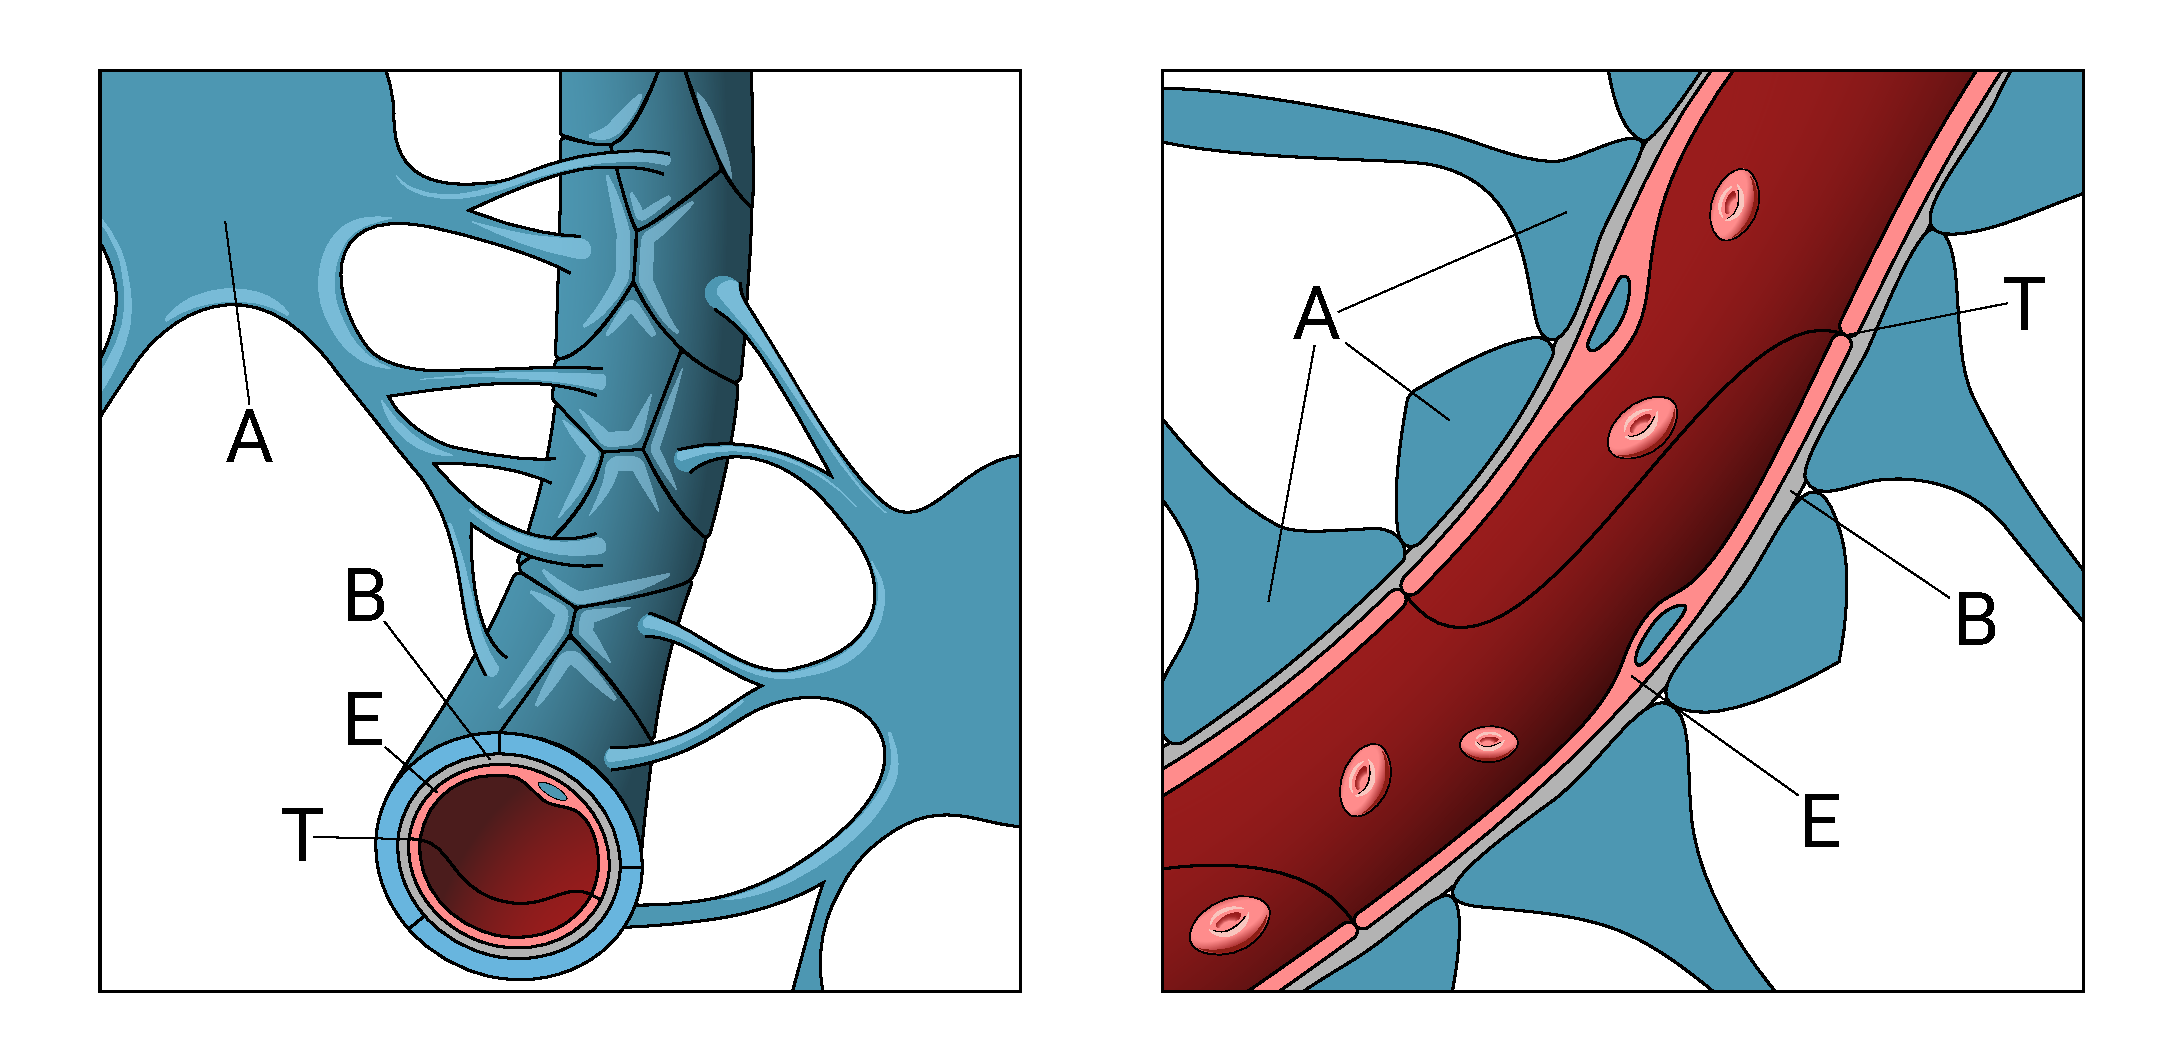
\includegraphics[width=\textwidth]{figures/bbb}
\caption[The blood-brain-barrier.]{\textbf{Schematic display of the blood-brain-barrier.} The blood-brain-barrier surrounds virtually every capillary in the CNS. A: Astrocyte, B: Basal Membrane, E: Endothelial Cell, T: Tight Junction. Modified from Lobentanzer \& Klein, 2019\cite{Lobentanzer2019b}.
\label{fig:bbb}}
\end{figure}

Before the advent of single-cell \ac{seq}, studies that endeavoured to clarify the transcriptional profiles of neurons used microarray technology, which was recently succeeded by \ac{seq} (also known as deep sequencing or next generation sequencing). For these methods, several cubic millimetres of brain tissue are required at the least; often, cubic centimetres are used. In contrast, the diameter of neuronal somata is usually in the micrometre range. Thus, the resolution of the method and the actual cellular resolution differ by a factor of approximately \num{10000}. Additionally, even among the neuronal population, there is considerable heterogeneity and transcriptomic plurality; single brain regions rarely consist of less than 30 different neuron types, tightly packed next to each other, each with their own transcriptional identity\cite{Darmanis2015, Zeisel2015, Tasic2016, Habib2016}. Newest studies, deciphering the murine nervous system by sequencing of \num{500000} individual cells, show that neuron diversity is very similar regardless of brain region\cite{Zeisel2018}. These circumstances hold true for any mammal, and most of our knowledge stems from the analysis of our favourite research animal, the mouse. In humans, the complexity is only exacerbated; in fact, the elevation in \ac{cns} transcriptional complexity might be the reason for our superior cognitive abilities(cite).

Cholinergic neurons always constitute a minority in any neuronal population, sometimes to extremes. Most tissues are dominated by few neuron types, such as pyramidal cells in the cortex; the most common neurotransmitter types are GABAergic (inhibitory) and glutamatergic (excitatory), each with several subtypes. It is estimated that more than 80\% of cortical neurons are excitatory, and more than 90\% of synapses release glutamate\cite{Raichle2002}. The striatum is fairly well-populated with rather large cholinergic interneurons, and the basal forebrain holds a large amount of (smaller) cholinergic projection neurons (compare Fig. \ref{fig:projections}). However, in transcriptomic analyses, these tissues are seldom used, for lack of scientific interest, or because they are notoriously hard to access (the basal forebrain is small and deeply imbedded in the midbrain). The cortex, particularly the neocortex, is most often the tissue of choice in these studies, due to its scientific interest and accessibility. Though it contains only a minuscule amount of cholinergic interneurons whose identity still is a matter of debate, several of the recent single-cell \ac{seq} approaches have independently identified cholinergic interneurons in cortical regions (see Fig. \ref{fig:singlecell}). 

All of the above taken into consideration, several limitations apply when it comes to the selection of a cellular model for the cholinergic processes we aim to understand. A multicellular model is prohibited by the novelty of the subject; possibilities include \textit{in vivo} or \textit{ex vivo} experimentation on rodents or human (3D-)cell culture with multiple cell types. While the former certainly is closest to reality, the diseases of interest display a noticeable lack of transferability from lower mammals to human(cite). The latter, on the other hand, introduces a complexity not well suited to the level of knowledge we possess about the studied processes; in addition, these models are very new, and thus, too many variables would be unknown. For these reasons, I selected two mono-cultures of human neuronal cells for my experiments. I chose to introduce a second cellular model during the experimental phase, because some of the studied diseases display a clear sexual dimorphism; the first experiments were performed on the female-originated LA-N-2 cell line, and later, to explore sex-related differences, the male-originated LA-N-5 cells were added.

\section{Cortical Single-Cell RNA Sequencing}
To estimate the potential impact of the transcriptomes studied in our model on the diseases of interest, co-expression of the relevant genes has to be asserted. Similarly, if neurokines are to possess any relevance for cholinergic properties of central nervous cells, the cells in question would have to express molecular machinery required to receive neurokine signals. The advent of single-cell \ac{seq} for the first time enables the resolution of gene expression on a cellular basis, and thus the disentangling of spatially close individual neuron types (and other, non-neuronal \ac{cns} cells); most of this information would be lost in \ac{seq} performed on brain homogenate, even of a small biopsy. Differences in genes would be reduced to the universally expressed »housekeeping« genes, and in \acp{mir}, the situation would be worse, in parallel to their even more tissue-specific expression.

For this reason, I analysed all publicly available single-cell \ac{seq} datasets relevant to our questions, which provide a detailed tally of transcriptional subtypes in the \ac{cns}. More specifically, all studies that were available at the time focused on some subsection of the cortex (visual or somatosensory) or the hippocampus. Additionally, the data provided by those studies was in some cases pre-aggregated to represent groups of single neurons with similar transcriptomes (Fig. \ref{fig:singlecell} A\&B\cite{Zeisel2015, Tasic2016}); in other cases, every single neuron was represented (Fig. \ref{fig:singlecell} C\&D\cite{Darmanis2015, Habib2016}). 

An important quality-related parameter of a single-cell \ac{seq} experiment is the sequencing depth achieved per individual sequenced cell. Some datasets I screened do not provide sufficient depth to resolve genes with medium expression, which includes our primary cholinergic markers \textit{\ac{chat}} and \textit{\ac{slc}}. The datasets which did provide adequate sequencing depth were filtered for their expression of these markers, and additionally characterised by their expression of common markers for cell types to be expected in the \ac{cns}. This resulted in a collection of transcriptomes for potentially cholinergic cells in the sampled brain regions, and allowed an assessment of the functional type and gene co-expression patterns in central cholinergic cells (Fig. \ref{fig:singlecell}).

\begin{figure}
\centering
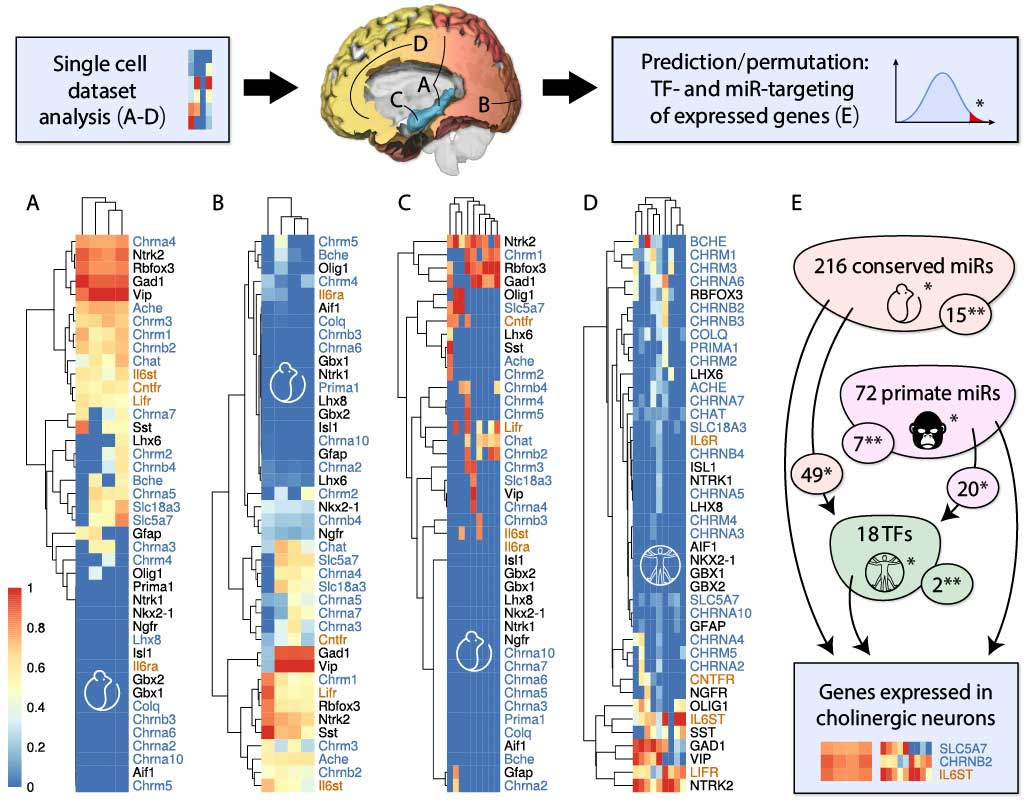
\includegraphics[height=10cm]{figures/singlecell}
\caption[Short figure name.]{This is a figure that floats inline and here is its caption.
\label{fig:singlecell}}
\end{figure}

Most cells identified as cholinergic by this definition expressed the general neuronal marker \textit{\acs{rbf}}, also known by its trivial name NeuN, but not the microglial marker \textit{\acs{aif}}. Few cells (or clusters of cells) expressed non-neuronal markers such as \textit{\acs{gfap}} (astrocytes) or \textit{\acs{oli}} (oligodendrocytes), hinting at sparse non-neuronal cholinergic functions. In agreement with my findings, cells or clusters identified as cholinergic by the authors of the respective studies had been classified as interneurons and co-expressed a number of known phenotypic neuronal markers, such as \textit{\ac{sst}} and \textit{\ac{vip}}.

The identified cholinergic cells also revealed a constant co-expression with neurokine-related genes, particularly the transmembrane neurokine receptors \ac{lifr} and \ac{ilst}, demonstrating a capacity to receive and process neurokine signals. In contrast, the high affinity receptor for \ac{ngf}, \textit{NTRK1}, is not expressed by many of the cholinergic neurons, fundamentally distinguishing these cells from the basal forebrain cholinergic projection neurons.
\todo{Clusters?}\todo{Permutation targeting analyses?}

\section{The Cellular Model}
\subsection{Requirements of a Cholinergic Neuron Cellular Model} \label{sec:cellculture:model}
Describe here the preliminary computational analyses leading to discovery of the CHAT miRNA anomaly, and thus the search for a CHAT-centric cell model? \todo{where goes the preliminary analysis?}
\subsection{The SH-SY5Y Neuroblastoma Cell Line}
A prominent example of human neuronal cell culture used in the identification and elucidation of cholinergic processes is the immortalised neuroblastoma cell line SH-SY5Y\cite{Biedler1978}. Derived from its parent line SK-N-SH, an adrenergic neuroblastoma\cite{Biedler1973}, it expresses ample amounts of \textit{\ac{ache}}, and thus had become a work horse in many cholinergic fields, such as Alzheimer's Disease (which is treated with \ac{ache} antagonists), pesticide development, and warfare(cite). However, in spite of its usefulness for processes involving \textit{\ac{ache}}, it turned out a less than optimal choice for the study of molecular events surrounding \textit{\ac{chat}} and \textit{\ac{slc}}, as it barely expresses both genes(cite), and cannot be coerced to elevate \textit{\ac{chat}} expression by the usual differentiation techniques (own experimentation, data not shown). Thus, for the questions asked in due course of this dissertation, SH-SY5Y does not qualify as adequate representation of a »cholinergic neuron«.

\subsection{The LA-N Neuroblastoma Cell Lines}
Following the elimination of SH-SY5Y as a suitable subject, I scoured the literature for candidates representing a cholinergic neuronal transcriptome, and found, among others, representatives of the LA-N neuroblastoma cell lines developed by R.C. Seeger around 1980\cite{Seeger1977, Seeger1982}. Neuroblastoma is a form of neuronal cancer often affecting small children, and, consequentially, the two cell lines used in my experiments are immortalised biopsies of a 3 year old girl (\acs{la2}\cite{Seeger1977}) and of a 4 month old boy (\mbox{\acs{la5}}\cite{Seeger1982}). The decision to use \ac{la2} as my initial cellular model was influenced by three factors: it is well described in literature, although most studies had been published in the 1980s and 90s; it expresses a substantial amount of \textit{\ac{chat}} and \textit{\ac{slc}}; and it responds to neurokine-mediated differentiation by assuming a neuronal morphology accompanied by further elevation of \textit{\ac{chat}} and \textit{\ac{slc}} expression. \ac{la5} was not nearly as well described as \ac{la2}, but later added to the experimental roster because of the complementary sex and hints towards cholinergic differentiation under retinoic acid\cite{Hill1997}.

\subsection{Culture}
LA-N cell culture is not as straightforward as many »go-to« human cell lines used in today's laboratories. Because \ac{la2} and \ac{la5} are very similar in this regard, they were treated similarly and I will describe the procedure for both. They have comparatively high duplication times, which can be lowered by using certain conditions that affect medium composition, nutrition, and CO\textsubscript{2} content. The cells were acquired at DSMZ (Braunschweig, Germany), which recommends keeping them in a 50:50 mixture of \ac{dmem} and \ac{rpmi}, with 20\% \ac{fcs} added. Sometimes, recommendations also suggest Leibovitz's L-15 medium, which is specifically designed for low CO\textsubscript{2} conditions, and others have suggested increased CO\textsubscript{2} levels inside the incubator. I found a combination of the DSMZ-recommended medium with 8\% CO\textsubscript{2} atmosphere inside a 37°C incubator to accelerate growth to a degree that the cells could be split 1:3 to 1:4 in a weekly cycle. This protocol was used for all further experiments, which were performed between splits 2 to 8 after thawing of a batch from -80°C. All handling during maintenance and experimentation was performed under a laminar flow hood.

\subsection{Differentiation}
Neuronal differentiation of neuroblastoma cell lines has been performed in many instances, utilising a wide variety of differentiation agents such as the very general retinoic acid or 5-bromo-uracil, or very specific reagents, such as the neurokines \ac{il} and \ac{cntf}(cite). LA-N cells have also been described to react to a selection of these substances; however, due to the elevated interest in neurokine mechanisms, I chose to go ahead with a reagent from this group. Somewhat arbitrarily, I used \ac{cntf}, because upon my inquiry, James McManaman revealed in personal communication that the »\textit{\ac{chat}} development factor« that he had discovered\cite{McManaman1988} was, in fact, \ac{cntf}, which had never been published. Additionally, of the neurokines used for differentiation purposes, \ac{cntf} is best described in literature and easily acquired in dried form from Merck (Darmstadt, formerly SigmaAldrich, Germany). \ac{cntf} was resuspended in pure water to a concentration of \SI{25}{\micro\gram\per\milli\litre} and stored for experimentation in aliquots at -20°C.

LA-N cells are very sensitive to repeated temperature changes, which resulted in increased amounts of apoptotic cells following repeated removal from the incubator after seeding or medium changes during the experiment. For this reason, I chose to only add the differentiation reagent once, 24h after initial seeding of the cells into the wells of a 12-well-plate, and avoid further disturbances until the time of lysis. For the maximum duration of my experiments, 120h from seeding until lysis, the initially supplied medium was sufficient for survival.

Differentiation was performed in regular growth medium without changes in \ac{fcs} content, and \ac{cntf} was added to the medium after an initial growth period of 24h. Cells were seeded into 12-well plates at approximately \num{200000} cells/well, with 1 ml of growth medium. To determine the optimal amount of \ac{cntf} for differentiation, time-dose-curves were determined for both cell lines in a range from \SIrange{1}{100}{\nano\gram\per\milli\litre}. Here, I discovered the first pharmacological difference between \ac{la2} and \ac{la5}: the maximum of their cholinergic response to neurokine stimulation (i.e., an elevation in \textit{\ac{chat}} and \textit{\ac{slc}} transcription) occurs at different concentrations of \ac{cntf}. While \ac{la2} cells respond most strongly to \SI{100}{\nano\gram\per\milli\litre}, \ac{la5} cells show an »inverted u«-type dose response with a maximum around \SI{10}{\nano\gram\per\milli\litre} \ac{cntf} (Fig. \ref{fig:time-dose}). James McManaman, who studied LA-N differentiation thoroughly in the 1990s\cite{McManaman1991}, believes both lines to respond in an »inverted u«-type manner (personal communication); thus, I assume that the \ac{la2} response would also diminish at \ac{cntf} concentrations significantly higher than \SI{100}{\nano\gram\per\milli\litre}. I also suspect that CNTF concentrations could be significantly lowered by removal of the high amount of \ac{fcs} in the medium, however, that would likely require the use of a special serum-free medium, which would have to be established up front, and might have other, unforeseen consequences. \ac{cntf} concentrations around \SI{100}{\nano\gram\per\milli\litre} (i.e., pico- to nano-molar) are well within the physiological range of concentrations that the mammalian brain is able to reach by paracrine secretion via, e.g., astrocytes\cite{Sun2016}.

\begin{figure}
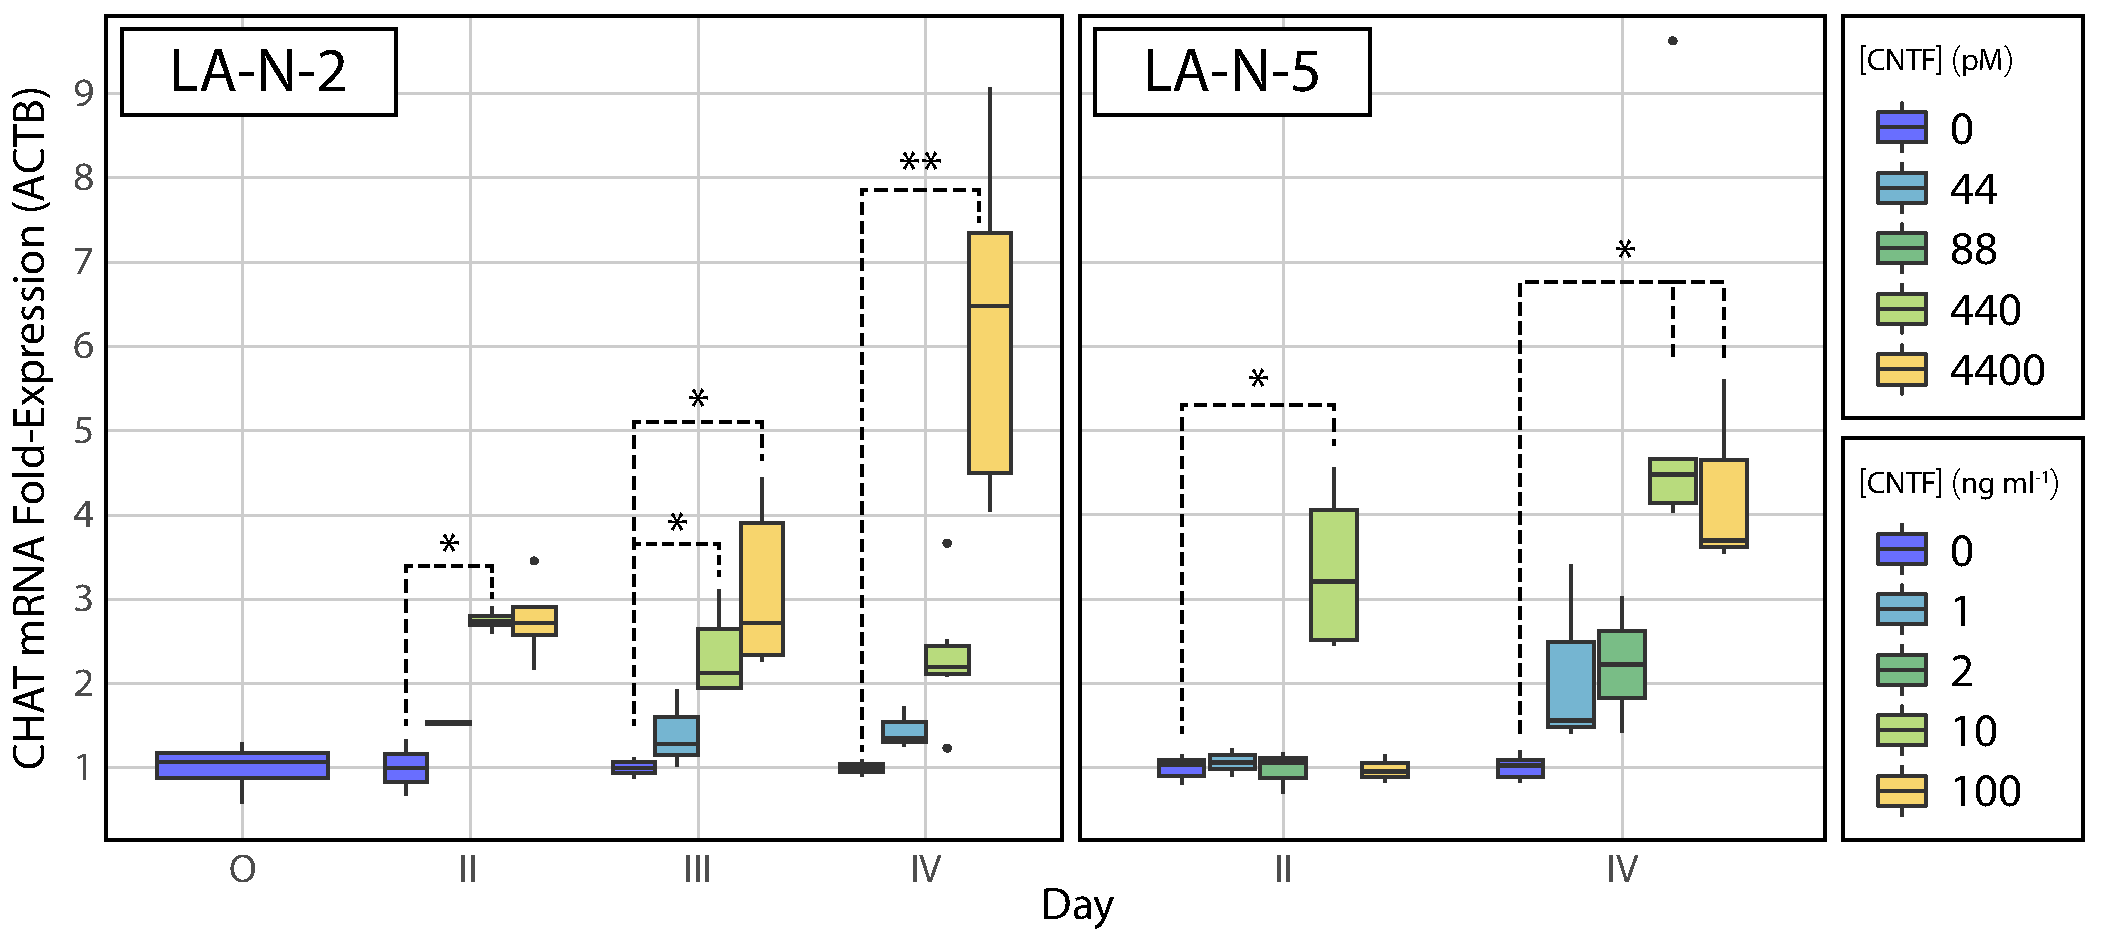
\includegraphics[width=\textwidth]{figures/time-dose}
\caption[Short figure name.]{This is a figure that floats inline and here is its caption.
\label{fig:time-dose}}
\end{figure}

To study the small RNA dynamics following \ac{cntf} exposure of \ac{la2} and \ac{la5}, I selected 4 time points at which the experiment was stopped and the cells were quickly lysed \textit{in situ} to preserve total RNA in that state: for the quick, immediate-early-like phase, at 30 and 60 minutes after the addition of \ac{cntf}, and, for the long-term effects of differentiation, at 48 and 96 hours after the addition of \ac{cntf} (Fig. \ref{fig:timepoints}, from my first publication\cite{Lobentanzer2019a}). Each time point was controlled by a pseudo-treated culture (using pure water) from the same batch that had been seeded at the same time as the experimental group. In the final series used for the parallel sequencing of \ac{la2} and \ac{la5}, all experiments were carried out in quadruplicates. 

\begin{figure}
\centering
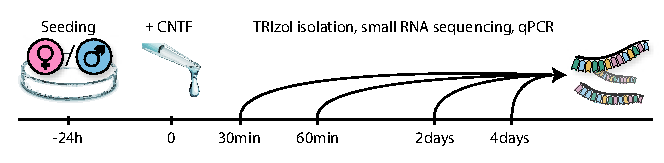
\includegraphics[width=0.8\textwidth]{figures/timepoints}
\caption[Short figure name.]{This is a figure that floats inline and here is its caption.
\label{fig:timepoints}}
\end{figure}

\subsection{RNA Isolation}
Total RNA was isolated using TRIzol (ThermoFisher Scientific), essentially as suggested by the manufacturer, with slight changes to the protocol to enrich small RNA species. The cells, growing in a monolayer in 12-well-plates, were cleared of medium, washed two times with \SI{500}{\micro\litre} of cell culture grade \ac{pbs} (Gibco), and immediately suspended in \SI{1}{\milli\litre} of TRIzol, pipetting up and down until visibly dissolved. After incubation for 5 minutes at room temperature, the samples were stored in -20°C for short periods of time until RNA isolation.

TRIzol-suspended lysates (\SI{1}{\milli\litre}) were added to RNA-separation centrifuge tubes (PhaseMaker Tubes, ThermoFisher Scientific), adding \SI{200}{\micro\litre} of pure chloroform and mixing vigorously for 15 seconds. After two minutes, the mixture was centrifuged at \SI{12000}{\g} and 4°C for 15 minutes, and the upper, watery phase containing the RNA was extracted. This was mixed with approximately 2 parts of pure ethanol and incubated for 10 minutes at room temperature to precipitate the RNA. The precipitate was spun at \SI{12000}{\g} and 4°C for another 10 minutes, and the supernatant discarded. The pellet was washed with 85\% ethanol (vortexed briefly) and centrifuged again for 5 minutes at \SI{7500}{\g} and 4°C.

After the final centrifugation step, the samples were transferred to the laminar flow hood, and air dried after removal of most of the supernatant via micropipettors. The pellet was allowed to dry almost until completion and resuspended in \SIrange{30}{50}{\micro\litre} pure RNase-free water. RNA concentration was measured at a Nanodrop 2000 instrument (ThermoFisher Scientific) and samples were diluted to a uniform concentration of \SI{100}{\nano\gram\per\micro\litre}. Finally, RNA samples were aliquoted according to later purpose and stored at -80°C.

RNA quality was determined by analysis on a 2100 Bioanalyzer instrument (Agilent) using a nano chip and \SI{1}{\micro\litre} of sample; \ac{rin} was near optimal for all samples ($> 9$).

\section{Small RNA Sequencing and Differential Expression Analysis}
For the detection and analysis of small RNA species, \ac{seq} is the current gold standard method. It allows the mapping of a comprehensive transcriptome and thus is vastly superior to small scale and consecutive methods such as \ac{pcr}. Assuming an adequate sequencing depth ($\gtrsim 1$ M reads/sample), it allows a comparison of all expressed small RNA species at once, which is immensely helpful when dealing with processes on the combinatorial scale of \ac{mir} regulation.

\subsection{Sequencing}
For small RNA sequencing, the aliquoted samples were shipped on dry ice to the cooperating institute at the Hebrew University of Jerusalem, the Silberman Institute of Molecular Biology, the laboratory of Prof. Hermona Soreq. \SI{600}{\nano\gram} of total RNA per sample were prepared for sequencing using the NEBNext Small RNA Library Prep Set for Illumina (New England BioLabs). The libraries were multiplexed with coloured barcodes, allowing for sequencing of all 48 samples on one chip. Briefly, this includes ligation of sequencing adapters to both 3' and 5' ends of all (single-stranded) RNA fragments in the sample, followed by 12-15 cycles of reverse transcription to form the RNA library. Ligated and amplified libraries were then size selected via gel electrophoresis on a 6\% Polyacrylamide gel. The band representing small RNA species on the gel was excised and prepared for loading onto the sequencing chip. After loading, the chip was sequenced in a NextSeq 550 series instrument (Illumina) with a read length of 80 bases, single-ended.

Sequencing quality was determined by analysis of the raw reads using the fastqc software(cite). \todo{describe quality parameters} \todo{examples?}

\subsection{Sequence Alignment}
Raw reads were adapter-trimmed and filtered for quality using the flexbar software(cite) with parameters \texttt{parameters here}\todo{parameters}. For the alignment of \ac{mir} sequences, parts of the miRExpress2(cite) pipeline were used in accordance to the documentation. This included the »Raw\_data\_parse«, »statistics\_reads«, »alignmentSIMD«, and »analysis« steps; »Trim\_adaptor« \todo{describe what miRExpress does?} was skipped because the adapters had already been trimmed in the quality filtering step. Additionally, since miRExpress is not accepting of sequences of any length, the raw data was length filtered to include only reads up to a length of 25 bases before input into miRExpress. Thus, raw reads were aligned to the miRnome provided by miRBase v21, yielding count tables of mature \acp{mir} and miRNA precursors for each sample. In total, XX \acp{mir} from miRBase v21 were discovered in the data.

\subsection{Differential Expression Analysis - R/DESeq2} \label{sec:cellculture:deseq}
To determine the effect and dynamics of \ac{cntf}-mediated differentiation of \ac{la2} and \ac{la5}, the expression state of each measured time point was compared to the respective control using the established R package DESeq2\cite{Love2014}. DESeq2 determines differential expression in count-based data by application of a linear regression model to a negative binomial distribution based on a fitted mean $\mu$ and a gene-specific dispersion value $\alpha$. The mean is derived using a sample-specific »size factor«, $s$, and a parameter $q$ proportional to the expected true concentration of RNA fragments in the sample. Thus, the DESeq2 differential expression pipline is composed of the following commands:
\begin{itemize}
\item \texttt{estimateSizeFactors()} (to estimate $s$)
\item \texttt{estimateDispersion()} (to estimate $\alpha$)
\item \texttt{nbinomWaldTest()} (application of a generalized linear model to determine log-fold changes and statistics via the Wald test)
\end{itemize}
The Wald test, named after Abraham Wald, is an approach to hypothesis testing that measures the distance between the tested unrestricted estimate and the null hypothesis, using the precision as a weighting factor. The larger the distance between tested values and the null, the more likely the measured values are »true«. \ac{seq} data can be modelled using binomial distributions\cite{Bullard2010}, such as the Poisson distribution, and the difference between two Poisson means (e.g., »treated« vs »control«) can be tested by generalised linear models based on the distributions themselves, Fisher's exact test, or the likelihood ratio test. However, comparative analysis has shown that the Wald test on log-transformed data provides statistical power superior to these other methods\cite{Chen2011}, particularly in lowly expressed fragments.

To reduce the noise introduced by the high variance in low-count genes while preserving large, »real« differences, the authors propose the »shrinkage« of log-fold changes to avoid arbitrary low-cut filtering at a predefined expression (count) value. Multiple variants are available; for \ac{mir} data, the adaptive algorithm »apeglm«\cite{Zhu2019} (adaptive t prior shrinkage estimator) yielded sensible results. \todo{example MDplots shrinkage?}

\subsection{microRNA Dynamics in CNTF-mediated Cholinergic Differentiation of LA-N-2 and LA-N-5}
Differential expression analysis performed in this manner yielded 490 \ac{de} \acp{mir} across all groups, with characteristic distributions between cell lines and time points. 

\subsubsection{Differential Expression in Both Cell Lines}

%\begin{wrapfigure}{r}{0.5\textwidth}
%  \begin{center}
%    \includegraphics[width=0.48\textwidth]{birds}
%  \end{center}
%  \caption{Birds}
%\end{wrapfigure}

114 mature \acp{mir} were detected as \ac{de} in both cell lines, with some changes similar in both, while others were inverted (Fig. \ref{fig:countchangecor}). In both cases, however, count-change values (see Box 1) correlated highly between the two cell lines (similar: 76 \acp{mir}, Spearman’s $\rho = 0.9066$, p < 2.2E-16; inverted: 38 \acp{mir}, $\rho = 0.9294$, p < 2.2E-16).

\begin{figure}
\centering
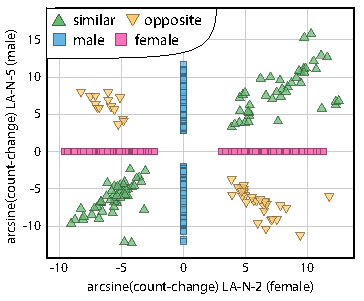
\includegraphics[width=0.5\textwidth]{figures/countchangecor}
\caption[Short figure name.]{This is a figure that floats inline and here is its caption.
\label{fig:countchangecor}}
\end{figure}

\begin{shaded}
\textbf{Box 1: The count-change metric.}

The frequently used log-fold change metric is not ideally suited for assessing the potential effect of expression changes for individual \acp{mir} because it does not reflect mean expression levels. To determine the absolute change in expression, I introduced the count-change metric, a combination of base mean expression and log-fold change, to weigh DE miRNAs against one another. The count-change is defined as follows: $$CC = (BM \cdot 2^{LFC}) - BM$$
CC: count-change, BM: base mean expression, LFC: log-2-fold-change.
\end{shaded}

\subsubsection{Differential Expression Along The Timeline}
Differential expression was detected in all groups, lending credibility to the rapid changes in expression needed for a \ac{mir} response of the »immediate-early« type (Fig. \ref{fig:timepointsexp}). However, the response to long-term \ac{cntf} stimulation was larger in \ac{mir} numbers as well as effect sizes. \todo{actual numbers} \todo{describe intersect to long term} \todo{compare most important targets short/long term}

\subsubsection{Differential Expression Between LA-N-2 and LA-N-5}
While there was considerable intersection between \ac{de} \acp{mir} between the cell lines (see above), a substantial amount of \acp{mir} was only \ac{de} in one of the two lines. Generally, response to \ac{cntf} was higher in the male-originated \ac{la5} cells; however, there were also \acp{mir} found \ac{de} only in the female \ac{la2} (compare Fig. \ref{fig:timepointsexp}). Thus, not all of the differences in \ac{mir} expression can be attributed to a higher sensitivity in \ac{la5}.

In total, 107 \acp{mir} were \ac{de} only in \ac{la2}, and 269 \acp{mir} were \ac{de} only in \ac{la5}. To categorise and systematise the sexual dimorphism of \ac{cntf} differentiation of LA-N cells, I performed gene set enrichment of \ac{mir} families in the differential expression datasets.

\begin{figure}
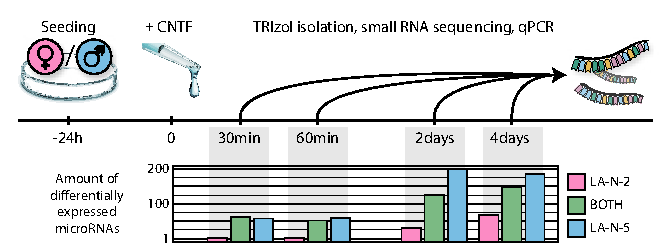
\includegraphics[width=\textwidth]{figures/timepointsexp}
\caption[Short figure name.]{This is a figure that floats inline and here is its caption.
\label{fig:timepointsexp}}
\end{figure}

\subsection{microRNA Family Enrichment}
Of the 151 \ac{mir} families listed in miRBase v21, members of 71 families are \ac{de} in \ac{la2} and \ac{la5}. To test for the enrichment of male, female, and ubiquitously \ac{de} \acp{mir} in these families, I performed gene set enrichment based on Fisher's exact test for each of the families. I found 5 families to be enriched in both male and female cells, and 12 families enriched in only one of the two cell lines (Fig. \ref{fig:mir-de-fam}, left side). The size range of enriched families was substantial, from small families with only 4 mature members to extensive families with dozens of mature \acp{mir}. 

\subsubsection{Gene Targeting of Enriched Families}
Using \textit{miRNet}, the targets of all individual \acp{mir} were determined, Of note, the amount of family members

\begin{figure}
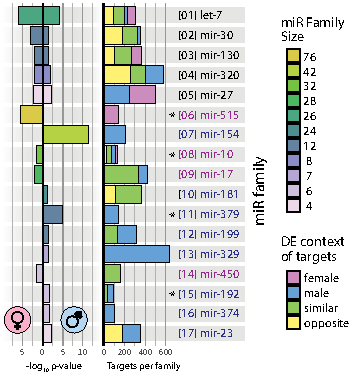
\includegraphics[width=0.5\textwidth]{figures/mir-de-fam}
\caption[Short figure name.]{This is a figure that floats inline and here is its caption.
\label{fig:mir-de-fam}}
\end{figure}

%\begin{table}
%\centering
%\begin{tabular}{c | c | c | c}
%family name & LA-N-2 p-value & LA-N-5 p-value & implicated in disease\\ \hline
%\hline
%let-7 & 1.2E-3 & 1.5E-7 & disease\\ \hline
%mir & pval & pval & disease\\ \hline
%\end{tabular}
%\caption{Enriched miRNA families in CNTF-induced differential expression in LA-N-2 and LA-N-5.}
%\label{tab:mir-de-fam}
%\end{table}

\section{Network Generation}

\section{The Cholinergic/Neurokine Interface}

\section{Application to Schizophrenia and Bipolar Disorder}

%!TEX root = ../dissertation.tex
\begin{savequote}[75mm]
I realized, "Oh my gosh! I'm having a stroke!" And the next thing my brain says to me is, Wow! This is so cool! How many brain scientists have the opportunity to study their own brain from the inside out?"
\qauthor{Jill Bolte Taylor}
\end{savequote}

\chapter{Dynamics Between Small and Large RNA in the Blood of Stroke Victims}

\newthought{Lorem ipsum dolor sit amet}, consectetuer adipiscing elit. Morbi commodo, ipsum sed pharetra gravida, orci magna rhoncus neque, id pulvinar odio lorem non turpis. Nullam sit amet enim. Suspendisse id velit vitae ligula volutpat condimentum. Aliquam erat volutpat. Sed quis velit. Nulla facilisi. Nulla libero. Vivamus pharetra posuere sapien. Nam consectetuer. Sed aliquam, nunc eget euismod ullamcorper, lectus nunc ullamcorper orci, fermentum bibendum enim nibh eget ipsum. Donec porttitor ligula eu dolor. Maecenas vitae nulla consequat libero cursus venenatis. Nam magna enim, accumsan eu, blandit sed, blandit a, eros.

\section{Background}
\section{Cohort}
\section{RNA Sequencing and Differential Expression Analysis}
\section{tRF Homology}
\section{WGCNA}
\section{Co-correlation}
\section{Networks}
\section{Direct Interaction}
\section{Feedforward Loops} \label{stroke:ffl}


%!TEX root = ../dissertation.tex
\begin{savequote}[75mm]
If the human brain were so simple that we could understand it, we would be so simple that we couldn’t.
\qauthor{Emerson M. Pugh}
\end{savequote}

\chapter{Discussion}

\newthought{Lorem ipsum dolor sit amet}, consectetuer adipiscing elit. Morbi commodo, ipsum sed pharetra gravida, orci magna rhoncus neque, id pulvinar odio lorem non turpis. Nullam sit amet enim. Suspendisse id velit vitae ligula volutpat condimentum. Aliquam erat volutpat. Sed quis velit. Nulla facilisi. Nulla libero. Vivamus pharetra posuere sapien. Nam consectetuer. Sed aliquam, nunc eget euismod ullamcorper, lectus nunc ullamcorper orci, fermentum bibendum enim nibh eget ipsum. Donec porttitor ligula eu dolor. Maecenas vitae nulla consequat libero cursus venenatis. Nam magna enim, accumsan eu, blandit sed, blandit a, eros.

\section{Methods} \label{sec:discussion:methods}
Quisque facilisis erat a dui. Nam malesuada ornare dolor. Cras gravida, diam sit amet rhoncus ornare, erat elit consectetuer erat, id egestas pede nibh eget odio. Proin tincidunt, velit vel porta elementum, magna diam molestie sapien, non aliquet massa pede eu diam. Aliquam iaculis. Fusce et ipsum et nulla tristique facilisis. Donec eget sem sit amet ligula viverra gravida. Etiam vehicula urna vel turpis. Suspendisse sagittis ante a urna. Morbi a est quis orci consequat rutrum. Nullam egestas feugiat felis. Integer adipiscing semper ligula. Nunc molestie, nisl sit amet cursus convallis, sapien lectus pretium metus, vitae pretium enim wisi id lectus. Donec vestibulum. Etiam vel nibh. Nulla facilisi. Mauris pharetra. Donec augue. Fusce ultrices, neque id dignissim ultrices, tellus mauris dictum elit, vel lacinia enim metus eu nunc.

\section{Small RNA Therapeutics and Pharmacology} \label{sec:discussion:therapy}
Extant approaches, methods, diseases, PCSK9, asthma, using small RNA antisense as substitute for single-target small molecules, reduce off-target effects, side effects of a different kind

Transcriptomics as basis for selection and design of antisense therapy, combinatorial, compare dirty drugs from psychiatric disorders, serendipity impossible, determinant is the sequence as opposed to functional groups that can be iteratively modified (only 4 building blocks)

%!TEX root = ../dissertation.tex
\chapter{Conclusion}
\label{conclusion}
The study of small RNA dynamics is greatly facilitated by modern bioinformatic methods that enable an understanding of complex transcriptional events in unprecedented detail. While the application and integration of the diverse sources characterising interactions and the participating molecules still are prone to error and misinterpretation, the field advances in giant steps. In summary, the dissertation here presented contributes to the field the following findings:

\begin{itemize}[noitemsep, leftmargin=.5cm, label={\tiny\raisebox{.5ex}{\textbullet}}]
\item Establishment of a framework for the fast and efficient computation of complex interactions between smRNAs, transcription factors, and target genes, including high-resolution tissue specific effects, and on the scale of the whole genome and all miRNAs and tRFs simultaneously;

\item (Re-)establishment of an \emph{in vitro} human cellular model for the study of cholinergic neurons with regard to sex specific phenomena, and, particularly, the effect of neurokine differentiation on cholinergic processes;

\item In this context, elucidation of the potential impact of small RNA dynamics in psychiatric diseases;

\item Identification of pertinent mechanisms in the response to stroke of blood-borne human cells, and interactions between small and large transcripts in these cells;

\item Identification of a neuro-immune axis connecting neurokine mechanisms and cholinergic signalling in multiple instances;

\item Exploration of the feasibility and practicality of feedforward loop analyses, in general and in an example of CD14$^+$ monocytes in post-stroke blood samples;

\item Description of a first step in utilising advanced network approaches for data science in the life sciences, for instance by implementing a »smart« dimensionality reduction.
\end{itemize}


\setstretch{\dnormalspacing}

%bibliography
\clearpage
\addcontentsline{toc}{chapter}{Bibliography}
\bibliography{library, manual_bib}
\bibliographystyle{mystyle}

% articles with multiple URLs have to be manually arranged in library.bib using »note = "\url{}"«
% maybe better just remove all but one URL

\clearpage
\addcontentsline{toc}{chapter}{List of Figures}
\listoffigures

%\clearpage
%\addcontentsline{toc}{chapter}{List of Tables}
%\listoftables

%appendix
\appendix
%!TEX root = ../dissertation.tex

\newcommand{\hsp}{\hspace{20pt}}
\titleformat{\chapter}[hang]{\huge\bfseries}{\textcolor{chaptergrey}{\thechapter}\hsp\textcolor{chaptergrey}{|}\hsp}{0pt}{\large\bfseries}
\titlespacing{\chapter}{0pt}{-40pt}{30pt}

\chapter{Transcription Factor Regulatory Circuits - Tissue Types} 
\label{appendix:marbach}

\begin{table}[ht]
\centering
\begin{tabular}{|l|l|}
	\hline
	\multicolumn{2}{|c|}{\bf CNS Tissues} \\
  \hline
  \hline
  AMYGDALA ADULT & NUCLEUS ACCUMBENS ADULT \\ 
  BRAIN ADULT & OCCIPITAL CORTEX ADULT \\ 
  CAUDATE NUCLEUS ADULT & OCCIPITAL LOBE ADULT \\ 
  CEREBELLUM ADULT & OCCIPITAL POLE ADULT \\ 
  CEREBRAL MENINGES ADULT & OLFACTORY REGION ADULT \\ 
  CORPUS CALLOSUM ADULT & OPTIC NERVE \\ 
  DIENCEPHALON ADULT & PARACENTRAL GYRUS ADULT \\ 
  FRONTAL LOBE ADULT & PARIETAL LOBE ADULT \\ 
  GLOBUS PALLIDUS ADULT & PONS ADULT \\ 
  HIPPOCAMPUS ADULT & POSTCENTRAL GYRUS ADULT \\ 
  INSULA ADULT & PUTAMEN ADULT \\ 
  LOCUS COERULEUS ADULT & SPINAL CORD ADULT \\ 
  MEDIAL FRONTAL GYRUS ADULT & SPINAL CORD FETAL \\ 
  MEDIAL TEMPORAL GYRUS ADULT & SUBSTANTIA NIGRA ADULT \\ 
  MEDIAL TEMPORAL GYRUS & TEMPORAL LOBE ADULT \\ 
  MEDULLA OBLONGATA ADULT & THALAMUS ADULT \\ 
  NEUROBLASTOMA CELL LINE &  \\ 
   \hline
   	\hline
	\multicolumn{2}{|c|}{\bf Immune Tissues} \\
  \hline
  \hline
  CD14-CD16+ MONOCYTES & LANGERHANS CELLS MIGRATORY \\ 
  CD14+CD16- MONOCYTES & LYMPH NODE ADULT \\ 
  CD14+CD16+ MONOCYTES & MACROPHAGE - MONOCYTE DERIVED \\ 
  CD14+ MONOCYTES & MAST CELL \\ 
  CD19+ B CELLS & NATURAL KILLER CELLS \\ 
  CD4+ T CELLS & NEUTROPHILS \\ 
  CD8+ T CELLS & SPLEEN ADULT \\ 
  DENDRITIC CELLS - PLASMACYTOID & SPLEEN FETAL \\ 
  ENDOTHELIAL PROGENITOR CELLS & THYMUS ADULT \\ 
  LANGERHANS CELLS IMMATURE & THYMUS FETAL \\ 
  \hline
  \multicolumn{2}{|l|}{CD34+ STEM CELLS - ADULT BONE MARROW DERIVED} \\
  \multicolumn{2}{|l|}{CD4+CD25-CD45RA+ NAIVE CONVENTIONAL T CELLS} \\
  \multicolumn{2}{|l|}{CD4+CD25+CD45RA+ NAIVE REGULATORY T CELLS} \\
  \multicolumn{2}{|l|}{CD4+CD25-CD45RA- MEMORY CONVENTIONAL T CELLS} \\
  \multicolumn{2}{|l|}{CD4+CD25+CD45RA- MEMORY REGULATORY T CELLS} \\
  \multicolumn{2}{|l|}{DENDRITIC CELLS - MONOCYTE IMMATURE DERIVED} \\ 
  \hline
\end{tabular}
\end{table}


%!TEX root = ../dissertation.tex
\chapter{List of Primate-Specific Homologues of Human microRNAs} 
\label{appendix:homologues}

%!TEX root = ../dissertation.tex
\chapter{microRNA Differential Expression in LA-N-2 and LA-N-5} 
\label{appendix:de-mirs}
%!TEX root = ../dissertation.tex
\chapter{List of GO Terms from Analysis of Differentially Expressed Large RNA in Stroke} 
\label{appendix:go-terms-large-rna}

%!TEX root = ../dissertation.tex
\chapter{Examples of Presence/Absence Definition of Small RNA} 
\label{appendix:presence-absence}


% the back matter
% \backmatter



% %!TEX root = ../dissertation.tex
\newpage

% If you do want an image in the colophon:
\begin{figure}
  \vspace{20pt}
  \centering
  \hspace*{-32pt}
  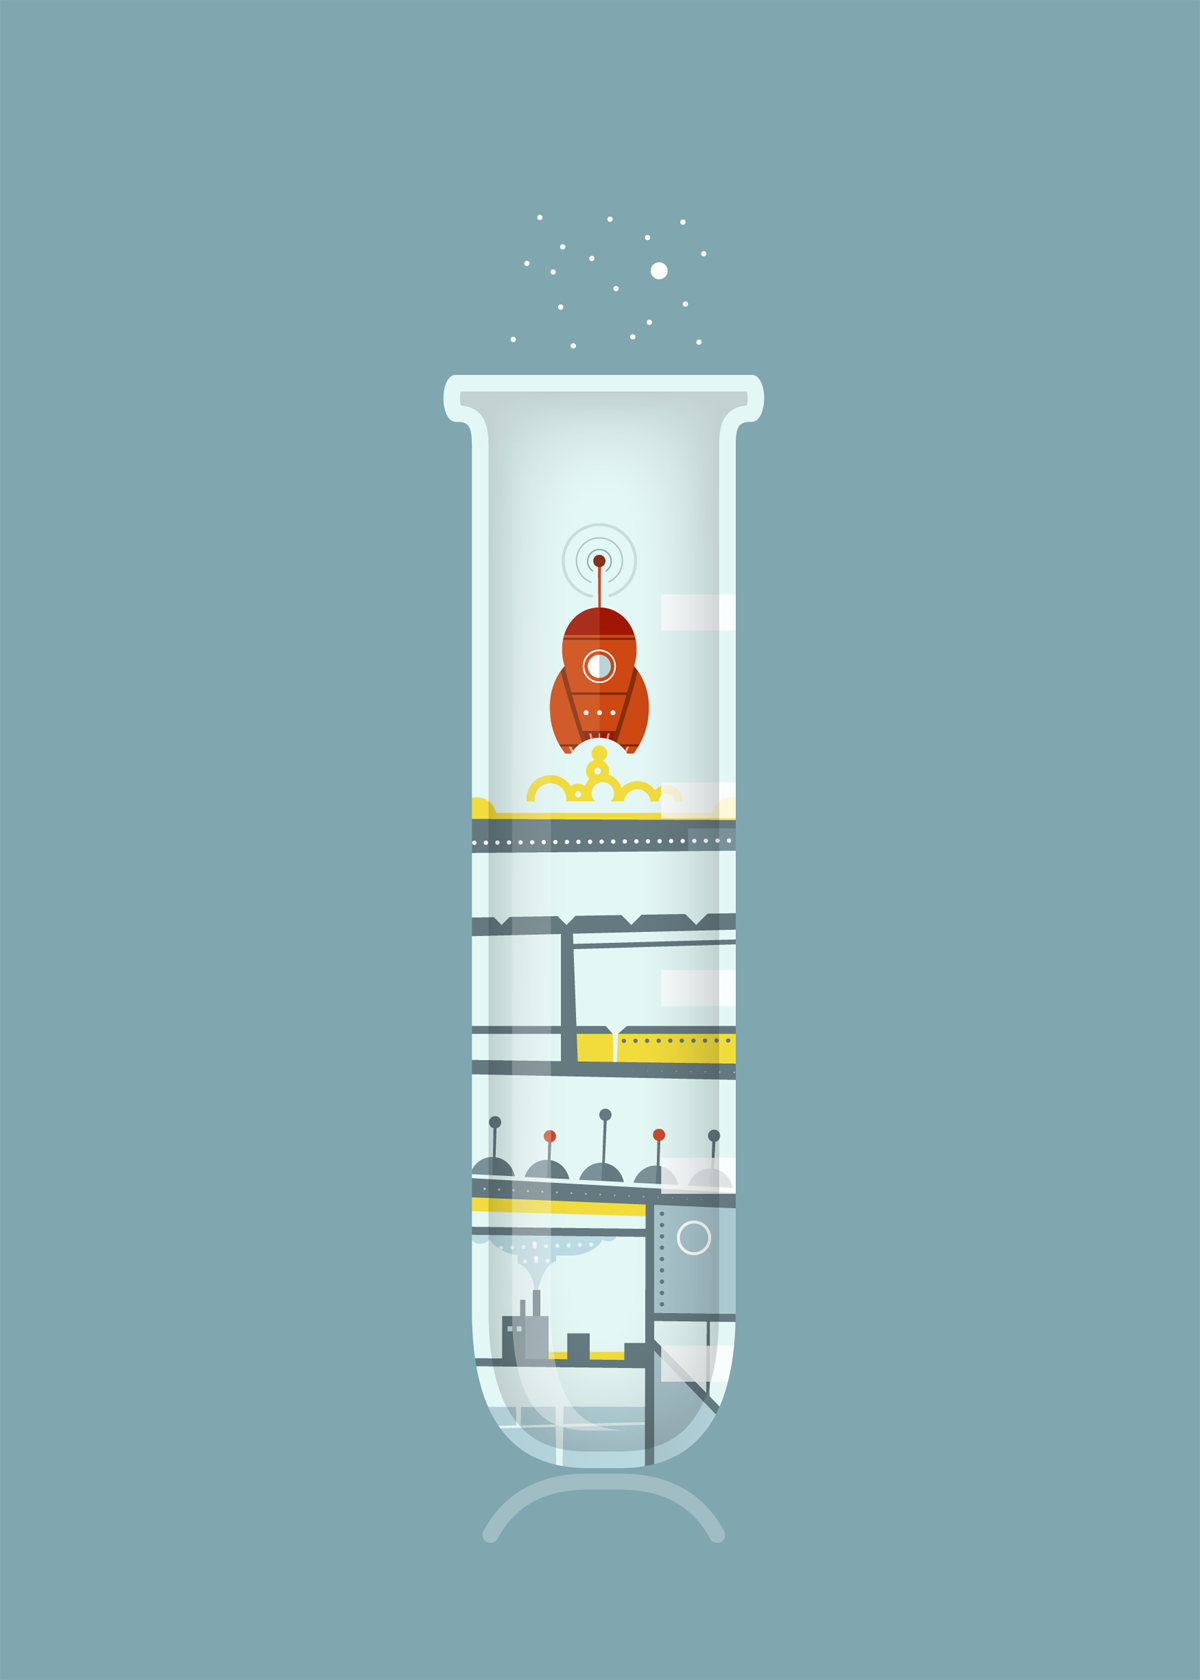
\includegraphics[width=0.42\textwidth]{endmatter/colophon.png}
\end{figure}

% If you don't want an image in the colophon:
% \vspace*{200pt}

\begin{center}
\parbox{200pt}{\lettrine[lines=3,slope=-2pt,nindent=-4pt]{\textcolor{SchoolColor}{T}}{his thesis was typeset} using \LaTeX, originally developed by Leslie Lamport and based on Donald Knuth's \TeX. The body text is set in 11 point Egenolff-Berner Garamond, a revival of Claude Garamont's humanist typeface. The above illustration, \textit{Science Experiment 02}, was created by Ben Schlitter and released under \href{http://creativecommons.org/licenses/by-nc-nd/3.0/}{\textsc{cc by-nc-nd 3.0}}. A template that can be used to format a PhD dissertation with this look \textit{\&} feel has been released under the permissive \textsc{agpl} license, and can be found online at \href{https://github.com/suchow/Dissertate}{github.com/suchow/Dissertate} or from its lead author, Jordan Suchow, at \href{mailto:suchow@post.harvard.edu}{suchow@post.harvard.edu}.}
\end{center}


\end{document}
